%%%%%%%%%%%%%%%%%%%%%%%%%%%%%%%%%%%%%%%%%%%%%%%%%%%%%%%%%%%%%%%%%%%%%%%%%%%%%%%%%%%%%%%%%%%
%%
%% LaTeX Template for Faculty of ICT at University of Malta
%%
%% The updated version of this document should be downloaded from
%%      https://github.com/jp-um/university_of_malta_LaTeX_dissertation_template
%%
%% In case of any difficulties please contact Dr JP Ebejer on jean.p.ebejer@um.edu.mt
%%
%%%%%%%%%%%%%%%%%%%%%%%%%%%%%%%%%%%%%%%%%%%%%%%%%%%%%%%%%%%%%%%%%%%%%%%%%%%%%%%%%%%%%%%%%%%

%% Before you embark on this quest you should probably read some of:
%% Deadly sins - http://mirrors.ctan.org/info/l2tabu/english/l2tabuen.pdf
%% Writing a thesis in LaTeX - http://tug.org/pracjourn/2008-1/mori/mori.pdf

\RequirePackage[l2tabu, orthodox]{nag} % tells you of any bad LaTeX usage
                                       % must be first thing in class (with the exception of comments)

%% There is one option you should define; oneside or twoside
%% Use twoside for your viva docs (examiners hate long docs they need to carry around)
%% and oneside for the final thing you submit to the library.  Note that margins will
%% change accordingly

\documentclass[oneside]{um-fict}  % custom University of Malta project/dissertation/thesis 


%% **************** (Your) Packages (Start) ******************

% \listfiles % uncomment this to know which packages you are using
              % the list of packages will be in the bottom of the .log file

%% Note that packges may already be loaded from the um (and memoir) classes.
%% Do not add your packages to the template, but rather add them here.

\usepackage{blindtext} %% for some dummy text, remove in your writeup
\usepackage{soul} % Remove in final version of document
\usepackage{amsmath} % for \text and \cases

%% ***************** (Your) Packages (End) *******************


%% **************** (Your) Data (Start) ******************

% A Comparative Study of Concurrent Queueing Algorithms & Their Performance
\title{A Comparative Study of Concurrent Queueing Algorithms \& Their\\ Performance}  % use \\ here otherwise you get a justified title
                                     % note capitalization of the title (only common 
                                     % words in lower case)
%\tagline{some hyped-up tagline}      % tag line
\author{Luca Muscat}            % your full name
\authorID{451401L}                   % your University Identifier
\supervisor{Prof Kevin Vella}              % your supervisor(s) name - no . in Dr
%\cosupervisor{Dr Who}                % your cosupervisor(s) name - no . in Dr *OPTIONAL* 
                                     % simply comment out the above line if absent

\degreeName{Bachelor of Science (Honours) (Computing Science)}       		 % the degree you are reading
                                     % note the \ after the dot, so not to consider it a fullstop
\doctype{dissertation}               % the type of document (fyp, dissertation, thesis)
\degreeDate{\monthyeardate\today}    % when did you submit (officially after your corrections)
%%\subjectcode{ICS5200}              % the study unit-code (currently not used)

%% ***************** (Your) Data (End) *******************


%% ******** (Your) Document Settings (Start) *************

% You should have an images directory in every chapX subdir
% NOTE:  Trailing / for subdirs is required.
\graphicspath{{./images/}{./chap1/images/}{./chap2/images/}}   % Paths where to look for images, if defined "images" must always be there as it holds the images in-use by the template.

\makeindex

%% ********* (Your) Document Settings (End) **************

% DOCTOR'S (JP) ORDERS: MAKE SURE TO READ MY TWO BLOG ENTRIES WITH
% CONTENT AND LaTeX TIPS FOR YOUR WRITE-UP.  THESE ARE BASED ON  
% EXAMINER'S FEEDBACK
%
% URLS:
% https://bitsilla.com/blog/2019/03/content-tips-for-your-dissertation-or-project-write-up/
% https://bitsilla.com/blog/2019/01/latex-tips-for-your-dissertation-or-project-write-up/

% end the preamble and start the document

\begin{document}
\frontmatter 
    \maketitle
%%    \begin{copyrightenv}
\end{copyrightenv}
       
%%    \begin{dedication}
{\large{To The Avengers}}\\[5mm]
You know, for saving the world.
\end{dedication}

        % include a dedication.tex file
    \begin{acknowledgements}
Firstly, my utmost appreciation goes to Prof Kevin Vella for his continual support,
which shaped and moulded this study to what it is today.

I would also like to thank my family for their encouragement, support, and for
filling the deep cavity in my coffee mug.
\end{acknowledgements}   % include an acknowledgements.tex file
    %% For tips on how to write a great abstract, have a look at
%%	-	https://www.cdc.gov/stdconference/2018/How-to-Write-an-Abstract_v4.pdf (presentation, start here)
%%	-	https://users.ece.cmu.edu/~koopman/essays/abstract.html
%%	-	https://search.proquest.com/docview/1417403858
%%  - 	https://www.sciencedirect.com/science/article/pii/S037837821830402X

\begin{abstract}
Queues are among the most ubiquitous data structures in the field of Computing
Science.
With the advent of multiprocessor programming, concurrent queues are at the
core of many concurrent and distributed algorithms.
Limited work related to surveying concurrent queueing algorithms and
replicating findings from their seminal works have been identified.
This work is an experimental study, with the aim of comparing performance
concurrent queues with one another under different levels
of contention, whilst replicating the results of other researchers. 
The production of a benchmarking framework for concurrent queues also forms
part of this study's contributions. 
We provide evidence to the fact that non-blocking queues are superior to blocking
ones under high contention, and remain competitive under low contention. We
also expose a number of unreported, yet significant biases in a number of
classical works. A limiting factor of this study is that each algorithm is
benchmarked on consumer-grade hardware, fortunately, the benchmarking framework
is developed to run on multiple machines, making this limitation transient in
scope.
Unbounded Multiple Producer Multiple Consumer (MPMC) queues are the focus of
this study.
\end{abstract}\if@openright\cleardoublepage\else\clearpage\fi
    \tableofcontents*\if@openright\cleardoublepage\else\clearpage\fi
    \listoffigures\if@openright\cleardoublepage\else\clearpage\fi
    %\listoftables\if@openright\cleardoublepage\else\clearpage\fi
    %%% will only print what is used ... useful.
%% also acronyms are clickable, which is awesome

\chapter{List of Abbreviations} %% \chapter*{List of Abbreviations} not to appear in LoC
\markboth{List of Abbreviations}{List of Abbreviations}
               
\begin{acronym}\itemsep-20pt\parsep-20pt %% if you remove these spacing params this list becomes huge!
\acro{CDMA}{Code Division Multiple Access}
\acro{GSM}{Global System for Mobile communication}
\acro{NAD+}[NAD\textsuperscript{+}]{Nicotinamide Adenine Dinucleotide}
\acro{NUA}{Not Used Acronym}
\acro{TDMA}{Time Division Multiple Access}
\acro{UA}{Used Acronym}
\acro{lox}[\ensuremath{LOX}]{Liquid Oxygen}
\acro{lh2}[\ensuremath{LH_2}]{Liquid Hydrogen}
\acro{IC}{Integrated Circuit}
\acro{BUT}{Block Under Test}
\acrodefplural{BUT}{Blocks Under Test}    
\end{acronym}
\if@openright\cleardoublepage\else\clearpage\fi

%% Note: always use \input as you cannot nest \includes (amongst other things)
%\pagestyle{umpage}
%\floatpagestyle{umpage}
\mainmatter 
    \chapter{Introduction}
\section{Problem Definition}
\section{Aims and Objectives}

A number of concurrent queuing algorithms, together with a benchmarking
framework are implemented in this study. In addition to the validation of results, all
measurements taken are compared amongst each other and their original works.
Thus, our objectives are the following:

\paragraph{\textbf{O1.}} Implement a benchmarking framework for concurrent queueing
algorithms capable of gathering measurements similar to prior works;

\paragraph{\textbf{O2.}} Reasonably validate the benchmarking framework through
metrics and experiments;

\paragraph{\textbf{O3.}} Implement a variety of concurrent queueing algorithms, with the aim
of replicating results from the original works.

\paragraph{\textbf{O4.}} Critically compare each concurrent queueing algorithm's performance
under a variety of synthetic benchmarks.
\section{Document Layout}
 
    \chapter{Background}

% [] Define what a multiprocessor environment is, and how it differs from a single processor environment.
% [] Define concurrent objects (using the text that already exists).
% [] Correctness conditions
% [] Progress conditions
% [] CPU Architectures, and why they should be taken into consideration.
% [] Mutual Exclusion

\section{Multiprocessors}
The diminishing growth in \emph{uniprocessor} speeds
forced programmers to look at parallelism as a means of improving
performance~\citep{cantrill2008real}. Unlike uniprocessors, \emph{multiprocessors} do
not ensure that instructions appear in execution order~\cite{scott2013shared},
making multiprocessors hard to model.

% \emph{Multiprocessors} consist of multiple hardware processors, each
% executing a \emph{sequential program}~\citep[Appendix~B.2]{herlihy2020art}.

Over the years, multiprocessor programming has become more practical and
feasible, partly thanks to multiprocessors getting cheaper, and
easier to program due to abstractions such as OpenMP, MPI (Message Passing
Interface), implicit parallel programming environments such as SQL, and
programming language standards that provide guarantees as to how parallel code will
behave, such as Java's\citep{javamemorymodel2014} and C++11's
\citep{cppmemorymodel} standardized memory models
\citep[Chapter~2.2]{perfbook2021}.

\emph{Multiprocessors} execute a number of \emph{processes} on distinct
hardware processors~\citep[Appendix~B.2]{herlihy2020art}, with each processor
continuously executing, and swapping out \emph{processes}.
\citeauthor{scott2013shared} defines a \emph{process} as a set of
\emph{threads}, where a thread is an active computation that has the potential
to share variables with other, concurrent threads~\citep[p.6]{scott2013shared}.
Once a process' \emph{time quantum} (fixed share of CPU time) expires, the
process is \emph{context-switched}. Processes
may be prematurely \emph{de-scheduled} due to interrupts,
system calls, or through the voluntary yielding of control to the CPU~\citep[Section~3.2.3]{osconcepts2021}.

% \citep[Appendix~B.7.1]{perfbook2021}.
For the sake of optimization, Compilers and CPUs do not guarantee specific
results in cases where multiple threads concurrently modify the same memory location~\citep{drepper2007every}. The explicit use synchronization primitives (such as read-modify-write operations
, or memory barriers) are needed to prevent incoherence
across caches, which may eventually lead to corrupt data.

\pagebreak

\section{Synchronization}
\subsection{CPU Cache}
As the disparity between CPU frequency and memory access times grew, 
CPU engineers added small, yet fast SRAM chips between the CPU
and main memory in order to alleviate issues caused by the differences in speed
~\citep{cantrill2008real,drepper2007every,perfbook2021}. Using large
quantities of SRAM is considered to be uneconomical, therefore, more cache layers
were introduced, with each layer being cheaper, larger, and slower than the
last~\citep{drepper2007every,perfbook2021}.

Data is transferred in units of \emph{cache lines}, which are power-of-two
fixed-size aligned blocks of memory, commonly ranging from 32 to 256 bytes in
size~\citep[Section~3.2.1]{perfbook2021}. Cache lines are filled with data
starting from the requested memory address, together with neighbouring bytes~\citep[Section~3.2.1]{perfbook2021}.

% The \emph{MESI} cache-coherence protocol (Modified, Exclusive, Shared, Invalid)
% attaches states to memory addresses; transitions notify the processor
% when to invalidate a cache line in order to prevent stale data~\citep[Appendix~B.5.1]{herlihy2020art}.

\emph{Cache-Coherence} is a problem where different caches contain stale
(out-of-date) values~\citep[Appendix~B.5.1]{herlihy2020art}. A memory address
may safely cached in different processors if no updates
occur; cache lines will be
invalidated if the contents of the shared memory address is updated (preventing
stale data from being read)~\citep[Appendix~B.5.1]{herlihy2020art}. The
\emph{MESI} cache-coherence protocol (Modified, Exclusive, Shared,
or Invalid) attaches states to memory addresses~\citep[Appendix~B.5.1]{herlihy2020art}. Transitions in
state notify the processor when to invalidate a cache line~\citep[Appendix~B.5.1]{herlihy2020art}.

%\emph{Sharing} occurs when overlapping data is loaded into several cache lines.
\emph{Sharing} occurs when one processor reads or writes to a memory address that
is cached by another~\citep[Appendix~B.5.1]{herlihy2020art}. In some cases,
sharing is unavoidable; closely located, yet
logically distinct data may share a single cache
line~\citep[Appendix~B.5.1]{herlihy2020art}. 

\emph{False Sharing} takes place when cache lines are invalidated due to updates
on logically distinct data~\citep[Appendix~B.5.1]{herlihy2020art}. As the
rate of invalidations increases with each write to shared-memory, performance
tends to degrade heavily, harming scalability. At the cost of a higher memory footprint, false
sharing may be solved by segregating logically distinct data with unused memory
to prevent the sharing of cache lines~\citep{scott2013shared}.

\subsection{Interconnection}

% TODO: Not really happy with the UMA definition, will need to give a better explanation.
An interconnection medium is used to connect CPUs to cache and memory; where
two kinds of interconnection architectures exist: (1)
\emph{Nonuniform memory access (NUMA)}
architectures~\citep[Appendix~B.3]{herlihy2020art} are typically associated with
multi-CPU and distributed systems; (2) \emph{Uniform memory
access (UMA)} architectures link processors and memory using a bus
interconnect~\citep[Appendix~B.3]{herlihy2020art}.

The cognizance of interconnection architecture is important,
as some algorithms are not suited for different architectures due to
overheads associated with accessing memory. This study will be
conducted on a \emph{UMA} architecture.

\subsection{Atomic Operations}
% TODO: Mention how CPUs can perform atomics semantically, as opposed to
% performing it in hardware.
% TODO: Find reference for the word size line.
An operation is said to be \emph{atomic}\footnote{Modern CPUs only guarantee
that atomic operations are semantically atomic, meaning that they do not
have to execute atomically on hardware.} if it is impossible to observe an
intermediate state~\citep{perfbook2021}. On most architectures, atomic
operations may only affect the CPU's word size worth of memory.

\emph{Read-Modify-Write (RMW)} operations read and write to memory
atomically~\citep{perfbook2021}. Most synchronization primitives may be
implemented as RMW operations~\citep[Section~5.6]{herlihy2020art}, and
typically need to be implemented in hardware~\citep[Appendix~B.8]{herlihy2020art}.
\citeauthor{herlihy1991wait} proved that not all synchronization primitives are
equally powerful by associating a \emph{consensus number} (i.e.~the number of
processes that the \emph{consensus problem} can be solved for) to each
synchronization primitive. \emph{Non-atomic} operations are prone to \emph{load} and \emph{store
tearing}~\citep[Section~4.3.4]{perfbook2021}\footnote{The Intel and ARM
architectures guarantee that correctly aligned loads and stores are
atomic~[\citealp{intel2021system},~Section~8.1.1;
\citealp{arm2022architecture},~Chapter~2.2].}.

\citeauthor{scott2013shared} lists a number of RMW operations~\citep[Table~2.2]{scott2013shared}.
\emph{Compare-and-swap} (\emph{CAS}, also known as \emph{Compare and Exchange})
is a ternary atomic operation that requires: A source, destination, and an
update value. If the source and destination are equal, the source is set to the
update value, otherwise, the destination is updated with the source's
value~\citep{intel2021inst}.
Older studies may give different definitions of
CAS~\citetext{\citealp{scott2013shared},~Table~2.2;~\citealp{valois1995datastructures},
Appendix~A}, such that line \ref{alg:line:sourceneqdest} is excluded.

\begin{algorithm}
    \caption{x86 compare-and-swap pseudocode.}\label{alg:cas}
    \begin{algorithmic}[1]
        \Function{compare-and-swap}{ptr<T> Source, ptr<T> Destination, T UpdateValue}
            \If{$Source~=~Destination$}
                \State $Source~\gets~UpdateValue$
                \State return True
            \EndIf
            \State $Destination~\gets~Source$ \label{alg:line:sourceneqdest}
            \State return False
        \EndFunction
    \end{algorithmic}
\end{algorithm}


\subsection{ABA Problem}
\citeauthor{dechev2010understanding} define the ABA problem as a false positive
execution of a CAS on a shared location~\citep{dechev2010understanding}. The ABA
problem may occur when the source's memory address has been changed from $A$ to
$B$, and back to $A$, bearing in mind that $A$ has been freed and immediately
allocated a logically distinct value, between the point in time when the
destination was loaded and the CAS was executed~\citep{dechev2010understanding}.

% [x] Caching is needed to avoid accessing slow memory by copying data into faster memory hardware
% [x] There are different levels cache, there is the register, L1, L2, and L3
% As cache levels move towards the register, access times get faster and cache sizes get smaller since they are more expensive.
% [x] CPU cache lines are used as a unit of transfer between different caches, on most architectures, a cache line is 64 bytes in size.
% [x] Mention what false sharing is and why it should be avoided.
% [] Mention how false sharing impacted this study's performance before being fixed.

\subsection{Progress Conditions}
A \emph{progress condition} is a \emph{liveness property} that describes how,
and when a number of threads are able to make \emph{forward
progress}~\citep[Section~3.2]{scott2013shared}.

A concurrent method is said to be \emph{blocking} if there is some reachable
state in the system where a thread cannot make progress until some other thread
takes action~\citep[Section~3.2]{scott2013shared}. Algorithms that rely upon
mutual exclusion are considered to be
blocking~\citep[Section~3.2]{scott2013shared}, however, non-lock-based
algorithms may also be blocking~\citep{mellor1987concurrent}.

A concurrent method is said to be \emph{non-blocking} if there is no reachable
state in the system where a thread cannot make
progress~\cite[Section~3.2]{scott2013shared}. The non-blocking property is
desired due to its immunity to random delays. % TODO: Find citation

The following are a subset of non-blocking progress conditions, ordered by the
strength of the property (starting from the weakest) and the complexity of
implementation (starting from the simplest):

\begin{enumerate}
\item \emph{Obstruction-Freedom}: A method is obstruction-free if, from any
point after which it executes in isolation, it finishes in a finite number of
steps~\citep[Section~3.8.3]{herlihy2020art};
\item \emph{Lock-Freedom}: A method is lock-free if some method call finishes
in a finite number of steps~\citep[Section~3.8.2]{herlihy2020art};
\item \emph{Wait-Freedom}: A method is wait-free if every call finishes its
execution in a finite number of steps~\citep[Section~3.8.1]{herlihy2020art}.
\end{enumerate}

Stronger guarantees do not necessarily equate to higher throughput, as the
overheads and complexity of the implementation tends to be positively
correlated to the strength of the guarantee.

\subsection{Correctness Conditions}
\label{sec:correctness_conditions}
\emph{Correctness conditions} describe the pre and post conditions for a concurrent
object's operations~\citep{herlihy2020art}. Such conditions decide
whether a concurrent history is legal \citep{herlihy1990linearizability}.
Correctness conditions are based on two requirements: (1) When an
operation takes effect, and (2) how the order of non-concurrent operations
should be preserved \citep{herlihy1990linearizability}.

A method is said to \emph{take effect} when the effects of its method call is
seen by other method calls~\citep[Section~3.4.1]{herlihy2020art}. 

% Find a formal definition of "takes effect"
\emph{Concurrent systems} may be modelled as a \emph{history}, which is a
sequence of events, where each event is either an \emph{invocation} or a
\emph{response}~\citep[Section~3.6.1]{herlihy2020art}. 

A history is said to be \emph{legal} with respect to a correctness property if
it is \emph{equivalent} to a history that respects said correctness property.

\citeauthor{lamport1979make} defines the \emph{sequential consistency}
correctness condition as a history in which the result of an execution is the
same as if the operations had been executed in \emph{program
order}~\citep{lamport1979make}.

A \emph{linearizable} concurrent computation gives the illusion that a method
call takes effect instantaneously some time between the method's invocation and
response; the point in time when the method takes effect is also known as the
\emph{linearizability point} \citep{herlihy2020art,herlihy1990linearizability}.
Processors perceive linearizable operations in a \emph{total, and real-time
order}, where overlapping method calls take effect in a non-deterministic
order~\citep[Section~3.6.2]{herlihy2020art}.


% [] What is a memory consistency model?
% [] Sequential Consistency
% [] Weak Consistency
% [] ARM is weakly consistent when writing to normal memory.
% [] Xbox360 CPUs are sequentially consistent as they reads and writes are in order (be careful, as in order might not be sequential consistence).
% [] Modern Intel CPUs use a variation of sequential consistency known as program-ordered-consistency

\subsection{Memory Consistency Models}
\emph{Memory Consistency Models (referred to as memory models henceforth)} are correctness properties that describe how
threads perceive the order of other threads' effects on shared
memory~\citep[Section~3.7]{herlihy2020art}. Similarly to the correctness
conditions described in section~\ref{sec:correctness_conditions}, memory
models vary in strength; as the model used becomes more relaxed, more aggressive
optimizations may be used, increasing performance at the cost of
programmability and portability~\citep{gharachorloo1996consistency}.

\emph{Relaxed memory models} such as \emph{weakly ordered models}\footnote{A number of ARM processors tend to be weakly ordered when interacting with main memory~\citep[Section~A3.5.5]{arm2022architecture}} offer little to no
constraints with respect to the ordering of reads and writes, requiring the
explicit use of memory barriers for a finer grained control over the ordering~\citep{gharachorloo1996consistency}. \citeauthor{gharachorloo1996consistency} identifies relaxed
memory models as \emph{system-centric models}, as they tend to favour
performance, as opposed to a programmer's intuition about shared-memory
(sequential consistency)~\citep{gharachorloo1996consistency}.

Memory models such as sequentially consistent models are considered to be
\emph{strongly ordered}. Strongly ordered systems tend to
heavily restrict the reordering of instructions, giving a simpler and
higher-level interface between memory and the programmer. 

\subsection{Mutual Exclusion}
\emph{Mutual exclusion} (also known as a \emph{mutex}, or a \emph{lock}) is a synchronization protocol that \emph{serializes}
the concurrent execution of code inside \emph{critical sections}.
A \emph{spin-lock} is a variant of a mutex, that 
\emph{busy-waiting}, and can be released by any thread.

Every mutex has to decide what actions to take when a
critical section has already been acquired; the three categories said action
can fall under are: 

\begin{itemize}
\item \emph{Blocking}~-~Voluntarily yields to the CPU
if the mutex is acquired. Blocking is not suitable for small critical
sections\footnote{A critical section is considered to be small if it takes
hundreds of nanoseconds or micro seconds to execute.}, as context switches typically take tens of milliseconds.
\item \emph{Busy-Waiting (spinning)}~-~Polls an area in memory
containing the state of a mutex. Busy-waiting is suited for small
critical sections, as contention caused by polling may lead to degraded
performance;
\item \emph{Hybrid}~-~Utilizes a mix of blocking and busy-waiting, forgoing the
inefficiencies associated with both methods.
\end{itemize}

Algorithms reliant on mutual exclusion are inherently
blocking (with respect to progress conditions)~\citep[Section~3.8]{herlihy2020art}, with
unique correctness conditions such as \emph{starvation} and \emph{deadlock
freedom}.

% TODO: Add a subsection on fairness

\section{Queues}
\citeauthor{knuth1968art} defines a queue as a linear list for which all
insertions are made at one end of the list and deletions are made at the
other~\citep{knuth1968art}. A queue comes with two operations, enqueue (places
an item at the head of the queue) and dequeue (removes and returns an item at
the tail of the queue), following First in First out ordering (FIFO).


\subsection{Concurrent Queues}
A concurrent queue is a type of queue that remains consistent and correct when
accessed simultaneously through different threads. Non-concurrent or
ill-synchronized queues typically end up in inconsistent states after being
accessed through multiple threads~\citep{yahav2003automatically}, leading
to hard-to-find bugs. Concurrent queues are often the basis of scheduling
algorithms~\citep{debattista2002high} and many other concurrent
algorithms~\citep{yahav2003automatically}. The defacto correctness condition
for a queue is linearizability, as it ensures that the semantics of the queue's
operations are not altered \citep{mellor1987concurrent, valois1995datastructures}.
% TODO: Add "Section 2.2.2" to valois1995datastructures reference

The multiplicity of the number of producers and
consumers that can simultaneously interact with a concurrent queue is used as a
taxonomy to categorize queues, furthermore, the underlying
data structure used to implement a queue (such as a circular buffer,
linked list, or both) affects if the queue is of \emph{fixed capacity (bounded)} or not
\emph{(unbounded)}. 

This study focuses on unbounded, MPMC, blocking and
non-blocking queues, with chapter \ref{chap:lit_review} covering the evaluated
queues in further detail.

\begin{table*}[h]\centering
\caption{Possible configurations in the Producer-Consumer taxonomy}\label{tab:producer_consumer}
    \begin{tabular}{lll}
        \hline
        Label & Description & Reference \\ \hline
        SPSC & Single-Producer/Single-Consumer & \citep{aldinucci2012efficient} \\
        SPMC & Single-Producer/Multi-Consumer & \citep{arnautov2017ffq} \\
        MPSC & Multi-Producer/Single-Consumer & \\
        MPMC & Multi-Producer/Multi-Consumers & \citep{michael1996simple,valois1994queues,hoffman2007baskets}\\ \hline
    \end{tabular}        
\end{table*}


% % When talking about correctness conditions with respect to FIFO queues, restricting the order of method calls is only a subset of the applicable correctness conditions. Yahav and Sagiv\citep{yahav2003automatically} provide some examples of correctness conditions for concurrent FIFO queues, which are:
% % \begin{itemize}
% %   \item The linked list is always connected
% %   \item Nodes are only inserted after the last node of the linked list
% %   \item Nodes are only deleted from the beginning of the linked list
% %   \item The head of the queue always points to the first node in the linked list
% %   \item The tail of the queue always points to a node in the linked list.
% % \end{itemize}

% \section{Mutual Exclusion}
% The 'Mutual Exclusion' protocol ensures that shared memory remains consistent when modified concurrently by two or threads running in parallel.

% % Mutual exclusion introduces the concept of critical sections, where different threads do not overlap \citep[Chapter~2]{herlihy2020art}. 

% Any mutual exclusion protocol needs to determine what to do when it is unable to acquire a lock. There are three alternatives to this problem \citep[Chapter~7]{herlihy2020art}:
% \begin{itemize}
%   \item Busy waiting - Conditionally and actively polls an area in memory or a shared resource. Busy waiting locks are typically referred to as spin-locks.
%   \item Blocking - Yields control of the CPU to other processes.
%   \item Hybrid - Makes use of both busy waiting and blocking for optimal use of resources.
% \end{itemize}

% ``Roll your own lightweight mutex''\citep{preshingmutex} covers a simple mutex implementation using a type of semaphore informally known as the `Benaphore'\citep{haikubenaphore}.

% ``Locks Aren't Slow; Lock Contention Is''\citep{preshinglockcontentionslow} offers insight into the performance of spin locks under contention. Preshing uses a custom implementation of the Mersenne Twister \citep{matsumoto1998mersenne} to simulate a critical section. The workload (ie. the amount of time that the lock is held for) and the number of threads used as variables whilst the lock frequency remained constant. The results show that high levels of contention on a lock is enough to degrade the performance of a parallel solution to the point where a sequential thread will perform better.

% Boyd-Wickizer et. al show that non-scalable locks, such as spin locks should not be used in operating systems where contention is hard to control. Several micro-benchmarks were implemented using a spin lock implementation offered by the linux kernel; as the contention increased, the performance of each benchmark dropped drastically. The spin lock was then re-implemented using scalable locks, such as the MCS lock \citep{mellor1991algorithms} and the CLH lock \citep{craig1993building,magnusson1994queue} improved performance on a large number of cores by at least 3.5 times, and in some cases, 16 times.

% Segall and Rudolph \citep{rudolph1984dynamic} propose an alternative to the test and set (TAS) spinning method called test-and-test-and-set (TTAS). TTAS reduces the amount of cache line invalidations caused by TAS spinning by checking if the flag being spinned on has changed before calling TAS.

% Anderson offers an improvement to the TTAS lock by implementing several spin locks based on CSMA network protocols \citep{anderson1990performance}. Anderson notes that spin locks using Ethernet's back off protocol tends to perform better under contention than a regular TTAS lock.

% Graunke and Thakkar also offer improvements to the TTAS lock by adding a delay after each failed test in order to reduce contention \citep{graunke1990synchronization}. The authors also proposed a novel queuing lock that outperformed all variations of the TAS lock when more than three processors are competing for access.

% Mellor-Crummey and Scott propose a novel array based lock known as the MCS lock that outperforms both array based queueing locks proposed by Anderson and Graunke et al. \citep{mellor1991algorithms}. The authors also offer insight into existing spin locks such as TAS, TTAS, and the ticket lock, and describe their benefits and their caveats.

% \section{Benchmarks and Performance Analysis Methodologies}
% Fog and McKenney offer insights into how to reduce the number of errors and interventions when micro-benchmarking \citep{fog1996optimizing,fog2020optimizing, perfbook2021}. Some measures to prevent errors are: keeping the CPU clock frequency stable (Stinner described methods of configuring and reading multiple CPU parameters \citep{stinnerpstate}), ignoring the first few iterations due to the cache and the branch predictor being cold\citep{fog1996optimizing}, avoiding symmetric multi-threading (aka. hyper-threading) \citep{fog2020optimizing} and detecting kernel interferences \citep[Chapter~11.7]{perfbook2021}.

% Intel's lock scaling analysis on Intel Xeon processors \citep{intelxeonlockscaling} benchmarks the relative contended performance of the Xeon Phi E5-2600 over X5600. The most notable contribution of this paper is the methodology used to for the benchmarks. The authors claim that a microbenchmark that aims to study lock performance does not reflect behaviour on real software if the study does not factor in the length of the simulated critical section and the frequency of locking. The paper reaches the conclusion that when predictable performance is desired, the locking algorithm requires reasonably long critical sections and re-entry times.

% Sahelices et al. offer a new methodology for tuning performance and critical sections inside of parallel programs \citep{sahelices2009methodology}. Critical sections were characterized by lock contention and degree of data sharing, allowing the authors to identify a number of inefficiencies caused by data sharing patterns and data layouts. Interestingly, the benchmarks were conducted on a multiprocessor simulator called RSIM, that allowed the authors to take fine grained and accurate statistics.

% Gregg describes several performance 'Anti-Methodologies' and 'Methodologies' \citep{methodologygregg}. Anti-Methodologies are methods of benchmarking performance that do not lead to accurate or correct results. This is an article that anyone in the field of performance analysis should read, as it reveals methodical and structured methods of carrying out performance analysis.

% Intel's optimization reference manual \citep{intelmanualoptimization} suggests several potential metrics that may be derived from specific hardware counters. Notably, equations for calculating bus utilization, L2 Modified Lines Eviction Rate, and Modified Data Sharing Ratio are all provided.

    %\chapter{Literature Review}
\label{chap:lit_review}

\section{Queues}
\subsection{\citeauthor{valois1994queues}' Queue}

\citeauthor{valois1994queues} surveys several lock-free data structures and
techniques \textemdash~ together with the introduction of the \emph{safe read}
memory reclamation scheme and an MPMC lock-free
queue~\citep{valois1994queues,valois1995datastructures}.
Combining the memory-reclamation scheme with the queue leads to increased cache line
churn, as enqueues traverse the queue's linked list for a bounded number of
nodes, causing each node's reference counter to be modified several times. 

% \citeauthor{michael1996simple} introduce the \emph{Two-Lock Concurrent} queue and the
% \emph{MS-Queue}~\citep{michael1996simple} \textemdash~a linked and concurrent
% queueing algorithm that is widely regarded as one of the most
% ubiquitous\footnote{Both \emph{Java\texttrademark's Concurrency
% Package}~\citep{java2022queue}, and \emph{Boost's Lock-Free
% Library}~\citep{boost2022queue} adopt the MS-queue algorithm.} lock-free
% algorithms in the field. Similar to \citeauthor{valois1994queues}' queue, the
% MS-queue uses disjoint head and tail references, together with
% the head always pointing at a dummy node~\citep{michael1996simple}. Thread
% helping is used as back-off technique that reduces contention from
% Compare-and-Swap.

\subsection{Michael's and Scott's Queues}

\paragraph{MS-Queue}
Similar to \citeauthor{valois1994queues}' queue, the MS-queue's head and tail
are separated, with the head always points to a dummy node. Compare-and-Swap
retry loops, which are a common pattern in lock-free algorithms, tend to
cause starvation and reduced parallelism.
\citeauthor{michael1996simple} adopt a thread-helping technique, where a thread
that fails to commit a node to the linked list, may help other threads by doing
part of their work, acting as a secondary back-off, reducing contention. 
The authors omit any discussion on the MS-queue's memory reclamation scheme,
which is a vital detail as pointed out by \citeauthor{michael2004hazard}
in \citep{michael2004hazard}, may lead to race conditions. 

\paragraph{Two-Lock Queue}
Similar to the MS-queue, the head and tail are separated, allowing for
concurrency between enqueues and dequeues~\citep{michael1996simple}. The ABA
problem does not exist in this algorithm, as Compare-and-Swap is not used;
furthermore, complex memory reclamation schemes are not needed, as access to
nodes are mutually exclusive, ensuring that a node may never be freed when
referenced by another thread.

\subsection{Optimistic MS-Queue}
\citeauthor{ladan2008optimistic} improve upon the MS-queue by enabling enqueues
to take effect in a single Compare-and-Swap~\citep{ladan2008optimistic}.
Enqueues add nodes to the beginning of the list;
doubly-linked lists allow for deleting nodes in the linked-list through backwards
traversals;
pointers to previous elements are maintained using simple stores, and are fixed
upon entering an inconsistent state (hence the \emph{optimistic} replacement of
Compare-and-Swaps).

\subsection{\citeauthor{hoffman2007baskets}'s Baskets Queue}
\citeauthor{hoffman2007baskets} present a variation of the MS-queue~\citep{hoffman2007baskets}, which is formed
using baskets (groups) of overlapping linearizable operations, which are non-deterministically
ordered among one another.
Time spent backing off in Compare-and-Swap failing threads is
spent inserting nodes into a basket, increasing parallelism across enqueuers;
the baskets mechanism also doubles down as a secondary back-off, further reducing contention.

Tagged pointers are used for ABA avoidance; dequeued nodes are logically
deleted by setting a flag bit packed inside the node's ABA counter. 
As the number of logically deleted nodes grows greater than the number of
\emph{max hops} (an arbitrarily chosen constant), or a logically deleted node
points to the tail of the queue, the \emph{free-chain} method is used to swing
the queue's head to the next non-deleted node, and reclaims any logically
deleted node between the head and the tail.

Under high levels of concurrency, the authors boast of a 25\% performance
improvement when compared to the MS-queue.

\subsection{Memory Reclamation Schemes}
Although memory reclamation schemes are omitted in this study, a brief discussion
on the field is essential to understanding the potential biases and discrepancies caused
by the omissions.

\subsubsection{Safe Read}
\emph{Safe Read}~\citep{valois1994queues,valois1995datastructures} 
is a reference counting memory management scheme that protects multiply referenced
pointers from ill-timed reclamation. 
Unlike the pointer packing technique, safe read reliably avoids ABA problems through
single-word Compare-and-Swap operations. \citeauthor{michael1995correction} discover
and correct race conditions in the \emph{safe read} protocol, that are liable to
corrupting and making unbounded use of bounded memory~\citep{michael1995correction}.

\subsubsection{Hazard Pointers}
\citeauthor{michael2004hazard}~\citep{michael2004hazard} presents a wait-free
memory reclamation methodology known as \emph{hazard pointers}

\section{Related Work}
Wait-free queues offer benefits such as starvation freedom and predictable
operation latencies \textemdash~at the cost of performance, practicality, and complexity.
Based on the MS-queue, \citeauthor{kogan2011wait} introduce one of the first practical unbounded, MPMC
wait-free queues~\citep{kogan2011wait} (henceforth known as the KP-queue). The
same authors present a methodology to create fast wait-free queues~\citep{kogan2012methodology} by
making use of the \emph{fast-path-slow-path} methodology; a lock-free queue is
used as the \emph{fast-path}, using a wait-free queue as a \emph{slow-path} after a number of failures.
used as the \emph{fast-path}, using a wait-free queue as a \emph{slow-path} after a number of failures.

    \chapter{Design \& Implementation}

\section{Relevant Software Versions}
Source code was compiled in the C programming language, using the clang
[version] compiler with flags `-O3 -march=native`\footnote{As opposed to the
gcc compiler, clang emits the \emph{cmpxchg16b} instruction without any extra flags.}. A number of researchers
utilize languages with heavy runtimes~\citep{kogan2011wait}, such as Java's JVM,
in order to shift the responsibility of memory management to the garbage
collectors, instead of the algorithm itself (making the C language's
light-weight runtime a reasonable choice).

Arguably, implementations of non-blocking algorithms in lock-based, garbage
collected languages are not truly non-blocking. \citeauthor{fog2020optimizing} argues that heavy-runtimes
are to be avoided, as the cost of operating the runtime is
typically greater than executing the algorithm
itself~\citep{fog2020optimizing}.

\emph{PAPI (Performance Application Programming Interface)} was used to measure
the elapsed time in nanoseconds~\citep{terpstra2010papi}. Although an entire library for measuring time 
is overkill, PAPI also provides an interface for measuring and
sampling hardware counters, which was used during the development of this project.

\section{Algorithms Implemented}
This study focuses on four concurrent queueing algorithms:
\citeauthor{michael1996simple}'s Lock-Free Queue~\citep{michael1996simple};
~\citeauthor{michael1996simple}'s Two-Lock Concurrent
Queue~\citep{michael1996simple} (protected by a \emph{test-and-test-and-set-lock}~\citep{mellor1991algorithms}); \citeauthor{hoffman2007baskets}'s Baskets
Queue~\citep{hoffman2007baskets}; and \citeauthor{valois1994queues}' Lock-Free
Queue~\citep{valois1994queues}. Keen-eyed readers may realize that the chosen
queues are unbounded and MPMC.

Due to limited time, the dynamic memory management of non-blocking
data-structures is omitted, as it is an actively researched field which can fit
an entire dissertation in of itself~\citep{valois1995datastructures,michael2004hazard}.

Memory is allocated before each benchmark, as to avoid bastardizing
non-blocking progress conditions through the use of lock-based memory
allocation. Pre-allocating memory prevents the ABA problem (as memory addresses
may no longer be reused)~\citep{dechev2010understanding}, removes the overhead
of memory allocation in measurements, and forgoes the need of memory management
schemes, as memory is released at the end of the benchmark.

\subsection{ABA Avoidance}

\emph{Version tagging} is used for ABA avoidance (not to be confused with
ABA-Freedom)~\citep{dechev2010understanding}:
A \emph{counter} (also known as a \emph{tag}) is attached to a pointer, which increments with
each successful CAS. Comparisons between pointers that have the same address,
but do not match in tag value are expected to fail, as differing tag values hint
at the possibility of a change in logical data. Counters may overflow, leading to tags wrapping back
to their initial value, allowing for ABA violations to still occur (however,
the chances are practically close to zero).

% When should version counting with DWCAS be used
For systems with a significant number of processors (for instance multi-CPU NUMA
architectures), larger counters are required  to safely avoid the ABA problem.
The \emph{Double-Width Compare-and-Swap} instruction (\emph{DWCAS}, \emph{CMPXCHG16b} on
\emph{Intel x86\_64}) may be used to attach a 64 bit counter to a pointer; Intel
systems require that the pointer and counter are aligned to a 16 byte boundary.

\begin{lstlisting}[language=C,caption={Struct aligned to 16 bytes, as required by the DWCAS instruction.}]
struct tagged_ptr{
    void* ptr;
    uint64_t tag;
} __attribute__((aligned(16))) tagged_ptr;
\end{lstlisting}

% Introduce pointer packing/tagged pointers
Alternatively, systems that do not provide the DWCAS instruction, suffer from
an unacceptable degradation in performance due to DWCAS, or do not allow for
the modification of pointers may employ a single-word CAS, by attaching a
counter to the pointer itself (known as \emph{pointer packing}, or \emph{tagged
pointers}) through the use of masking and shifting. Intel x86\_64 architectures supports 64 bit pointers, however, the
architecture only makes use of the least significant 48 bits (known as the
\emph{linear address})~\citep[Section~3.3.7.1]{intel2021system}, allowing for
the most significant 16 bits to be used as a counter.

% Explain pointer packing flaws
Pointer packing is flawed: The range of values a 16 bit counter can hold ranges
from zero to $2^{17}-1$ (which may easily overflow); pointer packing is not
portable, as there is no guarantee that the endianess, or the linear address
size will remain the same; pointers may only be dereferenced in their canonical
form, meaning that the most significant 16 bits either need to be set to zero
(user-space pointer) or one (kernel-space pointer), as canonical faults will be
thrown when dereferencing a pointer.

\subsection{Nanosecond Accurate Delay}
% High-resolution timers typically tick at a granularity of microseconds
% \textbf{(find a citation)}, leaving considerable slack between nanosecond
% delays and the elapsed time in reality. 
% The benchmarking framework relies on
% nanosecond-accurate ($10^{-9} seconds$) delays as a means of controlling
% contention. 
Delays of arbitrary lengths can be placed between operations, in order to
control contention~\citep{valois1994queues}. High-resolution timers may be accurate up
to a number of microseconds ($10^{-6}$ seconds), requiring a custom delay
function for nanosecond accuracy ($10^{-9}$ seconds). With respect to CPUs,
time may be described in different dimensions,
where the number of CPU cycles can be extrapolated from wall-clock time and the
CPU's clock speed, allowing for an instruction, with a known latency, to be
executed as many times as required to consume an arbitrary number of
time. Unfortunately, extrapolating CPU cycles from wall-clock time
requires a fixed CPU clock speed, hurting the validity of results in cases
where CPU clock speeds are highly unstable.

% Drawing inspiration from \citeauthor{intel2013lockscaling}'s~lock
% scaling analysis on
% Xeon\textregistered~processors~\citep{intel2013lockscaling}, inter-arrival
% times are on the scale of nanoseconds.

Similar to \citeauthor{intel2018spinloop}'s
\emph{Architecture Agnostic Spin-Wait Loops}~\citep{intel2018spinloop} and
\emph{pollDelay} function~\citep[Example~2.3]{intelmanualoptimization}, a
nanosecond delay can be created by constantly polling the CPU's timestamp
counter, until the extrapolated number of cycles are
consumed~\cite{ramalhete2019delay}.

% uint64_t stop;
% uint64_t start = _rdtsc();
% do
% {
%     stop = _rdtsc();
% } while (stop - start < cycles);

\begin{algorithm}
    \caption{Delay implemented through polling the CPU's timestamp counter.}\label{alg:delay}
    \begin{algorithmic}[1]
        \Function{delay\_ns}{uint64\_t time\_ns}
            \State $cycles \gets time\_ns \cdot cpu\_frequency\_ghz$
            \Comment{Pre-calulate to prevent inaccuracies.}
            \State $start \gets read\_timestamp()$
            \Repeat
                \State $stop \gets read\_timestamp()$
            \Until{$stop - start < cycles$}
        \EndFunction
    \end{algorithmic}
\end{algorithm}

The delay's accuracy is significantly improved through calibration, where the
delay function is put through a trial run, and the number of cycles to be
executed are modified according to the error between the delay's average time
elapsed, and the expected delay.

\subsection{Test \& Test \& Set with Exponential Delay}


\section{Methodology}

% TODO: Can add more citations to this part; can be taken from the literature
% review once that's done.
Studies introducing novel concurrent
algorithms~\citep{michael1996simple,valois1994queues,kogan2011wait,hoffman2007baskets,yang2016wait}
frequently conduct comparisons between their novel and existing algorithms in
similar fashions. The most common benchmarks for evaluating concurrent queueing
algorithms are the \emph{Pairwise Enqueue Dequeue} and \emph{50\% Enqueue}
benchmark. As to amortize measurement overheads, ten million iterations are
executed amongst $N$ threads ($t_0,~t_1,~\cdots,~t_{N-1}$) as follows: 

\[
    \text{iterations(i)} = 
    \begin{cases}
        \lfloor\frac{10^7}{N}\rfloor, & \text{if}~i < N-1 \\
        10^7 - (\lfloor \frac{10^7}{N} \rfloor \cdot (N-1)), & \text{otherwise}
    \end{cases} \\
\]

for ten times, with the recorded sample being the average of the average
elapsed time from each thread for each repetition.

\subsection{Pairwise Enqueue Dequeue Benchmark}

On an initially empty queue, each thread enqueues an item, executes an
artificial delay (which \citeauthor{michael1996simple} refers to as "other
work"~\citep{michael1996simple}), dequeues an item, and executes another
artificial delay; The queue is destroyed and recreated with every repetition
(i.e. every ten millions iterations). \citeauthor{michael1996simple} uses an
artificial delay to reduce the bias introduced by long runs of queue operations
by a single thread~\citep{michael1996simple}. The number of threads, and length
of the artificial delay are used as the benchmark's independent variables, the
degree of contention is dependent on both the number of threads and the length
of the delay, furthermore, the measured time taken is also dependent on
contention and operating system activities. This benchmark serves the purpose
of simulating a producer-consumer workload, where each thread acts both as a
producer, and a consumer.

\subsection{50\% Enqueue Benchmark}
Each thread either executes an enqueue or a dequeue, with each operation
getting a 50\% chance of executing\footnote{Using a uniform distribution},
followed by an artificial delay, on a queue that is prefilled with 1000
elements. The queue is prefilled with 1000 items to prevent long runs of empty
dequeues (potentially introducing biases). Randomness aids with exercising a
larger number of code paths.

Random numbers are stored as double-precision floating point variables, ranging
from zero to one, furthermore, they are generated before the execution
of the benchmark, as to calculate the number of enqueues (consequently the
amount of memory that needs to be allocated), and to reuse the same random
numbers with every repetition, in order to maintain consistency. 

It is important to note that the 50\% enqueue benchmark will execute at most
half the number of enqueues and dequeues executed as the pairwise
enqueue-dequeue benchmark, as an operation is no longer executing a pair of
enqueues and dequeues, but either one of them.

A number of measures to reduce variance and
interference caused by the operating system are taken: Hyperthreading is
disabled, as it leads to higher rates of cache misses due to each core's cache
being split with another thread~\citep{fog2020optimizing}; The CPU's speed is
fixed to its maximum frequency by setting the CPU frequency governor to
\emph{performance} mode (using \emph{cpufreq-set -g performance}) in order to
restrict fluctuations in the CPU's clock speed, which may lead to inaccurate
measurements and delays at the cost of a higher energy cost; Turbo boost is disabled as it dynamically increases
processor performance according to the CPU's thermals~\citep[Section~14.3.3]{intel2021system}.

    \chapter{Evaluation}
In this chapter, insights emanating from each queue's evaluation is compared
with findings from their seminal works. Data gathered from the benchmarking
framework is used to characterize the performance of each queue.
Each section in this chapter will be dedicated to the performance of each
queue under a workload of a fixed number of threads, and varying
delay between queue operations.
A queue's performance is quantified using the net runtime of each benchmark,
together with the magnitude of performance degradation, which is
calculated as the ratio of net runtime between the current and previous thread
(where a value greater than one indicates degraded performance).

\section{Workload under one thread}

\begin{figure}[!ht]
    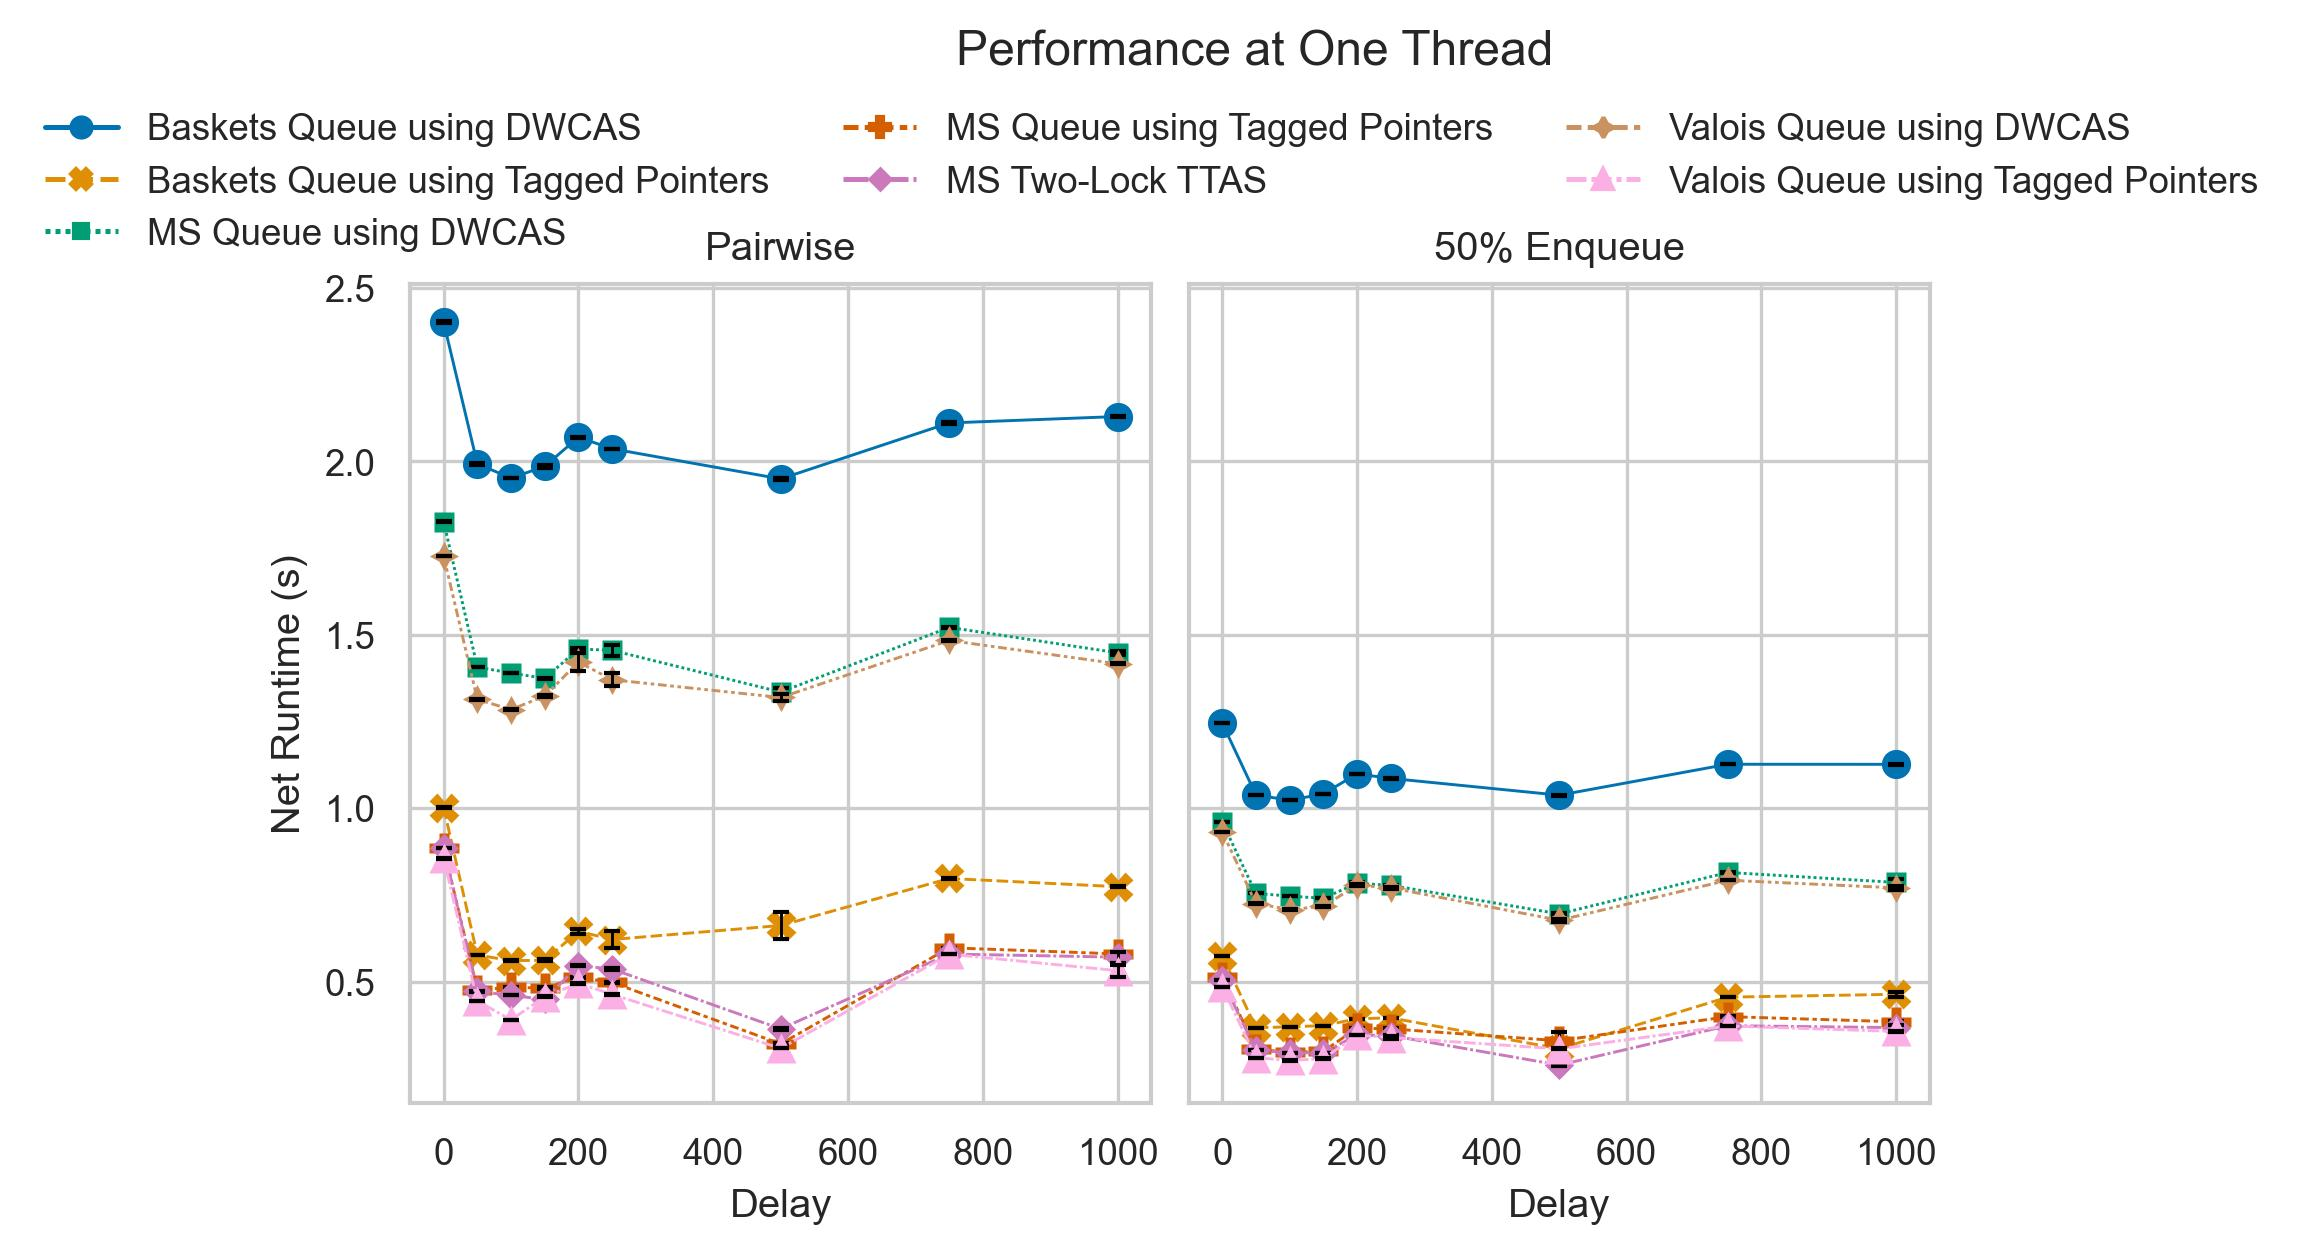
\includegraphics[width=1\textwidth]{plots/delay_thread_1.jpg}
    \caption{The pairwise and the 50\% benchmarks on the left and right respectively.}
    \label{fig:perf_1_thread}
\end{figure}

The sequential latency of a queue is determined by its algorithmic
complexity~\citep{valois1995datastructures}. Contention-reducing
mechanisms\textemdash such as thread helping\textemdash are not triggered under
single threaded workloads as they rely on failed CAS operations, adding
extra overhead through the computation of predicates.
Figure \ref{fig:perf_1_thread} shows the performance of each queue in a single
threaded workload. Under the \emph{pairwise benchmark}, the \emph{MS-Queue} and
the \emph{Baskets Queue} using tagged pointers are at most \textbf{3.168} and
\textbf{2.593} times faster than their DWCAS counterparts. 
The \emph{Baskets Queue} is consistently outperformed by the \emph{MS-Queue}
and the \emph{Two-Lock Queue} (respectively, at most \textbf{0.450} and
\textbf{0.516} times slower). Although the \emph{pairwise benchmark} does not
show which queue is consistently faster, the \emph{50\% enqueue benchmark}
shows that the \emph{Two-Lock Queue} consistently outperforms the
\emph{MS-Queue} (by at most \textbf{0.27} times).

\section{Workload under two threads}
Similar to \citep{michael1996simple,hoffman2007baskets,ladan2008optimistic},
under a workload of two threads, a significant degradation in performance can
be observed. \citeauthor{michael1996simple} notes that as each queue's head and
tail are shared across two processors, cache misses are more frequent. 
Figure \ref{fig:perf_deg_1_thread} shows that queues using tagged pointers tend
to experience higher contention, consequently leading to worse performance. 
In support of this claim, the \emph{Baskets Queue using Tagged Pointers} with
50 nanoseconds of delay was \textbf{2.435} times more likely to re-attempt an
enqueue\footnote{This metric was gathered by incrementing an integer (found in
thread local storage) every time it repeated anything past line \emph{E03} of
the Baskets Queue.} than its DWCAS counterpart.

\begin{figure}[!ht]
    \centering
    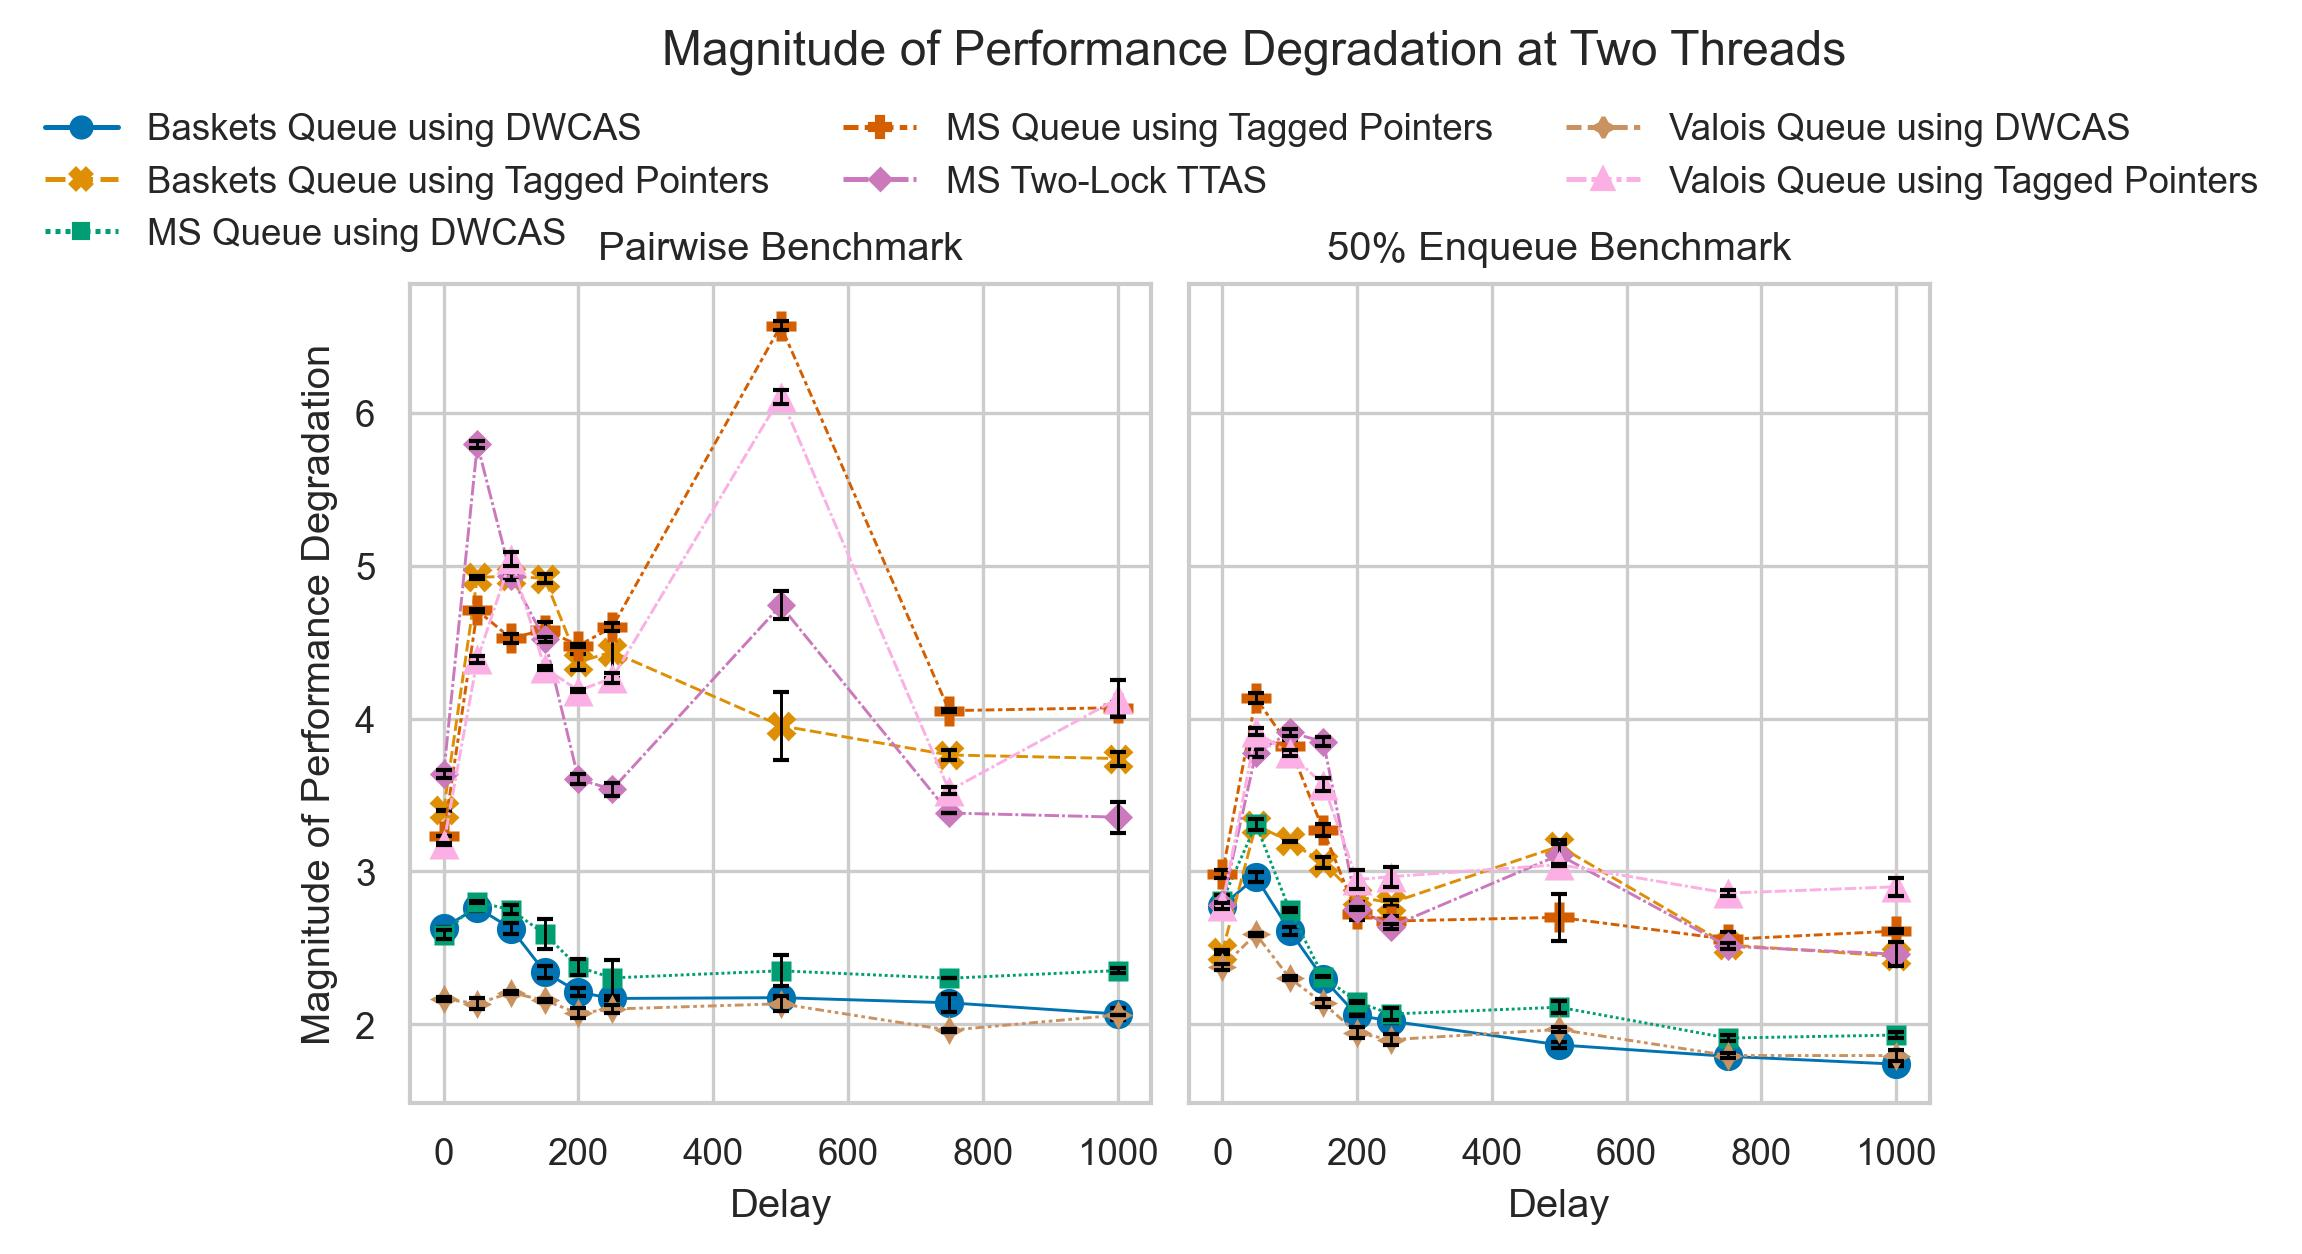
\includegraphics[width=1\textwidth]{plots/speedup_1.jpg}
    \caption{The magnitude of performance degradation between single and two-threaded workloads.}
    \label{fig:perf_deg_1_thread}
\end{figure}

\begin{figure}[!ht]
    \centering
    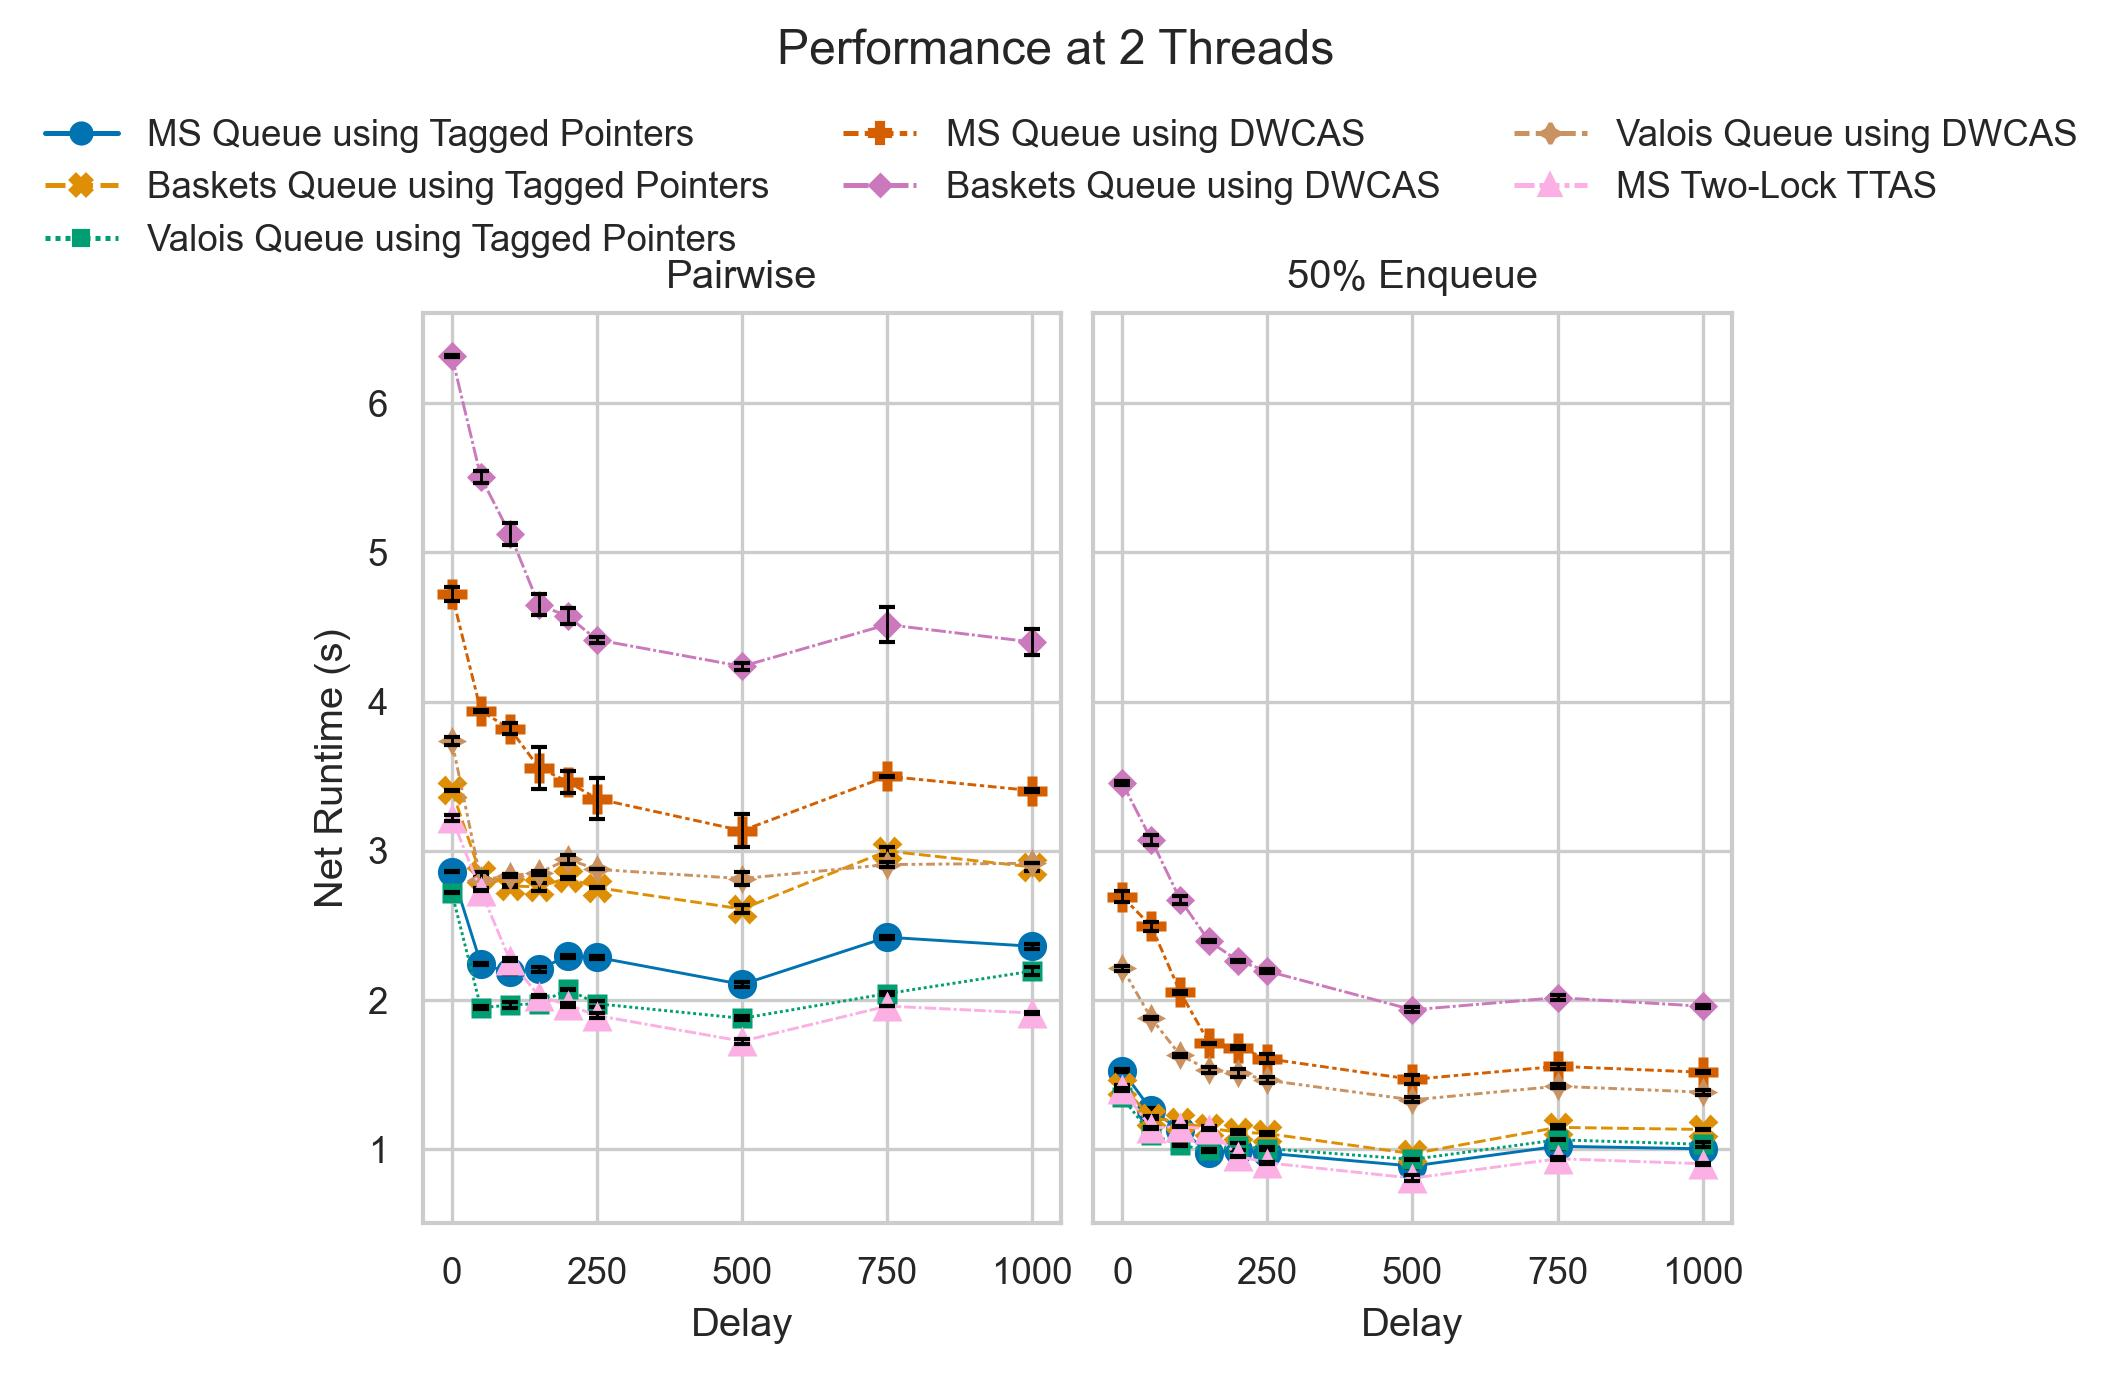
\includegraphics[width=1\textwidth]{plots/delay_thread_2.jpg}
    \caption{The pairwise and the 50\% benchmarks on the left and right respectively.}
    \label{fig:perf_2_thread}
\end{figure}

In the \emph{pairwise benchmark}, the \emph{Baskets Queue} is consistently
outperformed by the \emph{MS-Queue} and the \emph{Two-Lock Queue} by at most
\textbf{20.978\%} and \textbf{34.672\%}, with the \emph{Two-Lock Queue}
consistently outperforming the \emph{MS-Queue} by at most \textbf{11.100\%}.

At delays greater than 200 nanoseconds, the \emph{two-lock queue} exhibits the
best performance.
Although outperformed, non-blocking queues using tagged pointers remain
competitive under low-contention. 

The performance of \citeauthor{valois1994queues}' queue in this study highly
conflicts with that of \citep{michael1996simple}. Although a queue without a
memory reclamation scheme may share a common algorithm with one that has, it
does not imply that they are algorithmically equivalent, making their
performance unconnected; as this study does not include memory reclamation
schemes in its implementations, valid comparisons cannot be made with
~\citep{michael1996simple}'s results of \citeauthor{valois1994queues}' queue,
however, insights may still be inferred.
\citeauthor{michael1996simple} fail to disclose that their choice of
memory-reclamation schemes introduced a significant bias in favour of their
novel algorithms. 
This is only made clear when inspecting the study's published source
code~\citep{michael1996simple_sourcecode}, where \citeauthor{valois1994}' queue
makes use of the safe-read protocol, whilst the \emph{MS-Queue} only keeps
track of each threads' most recently recycled node non-atomically in thread
local storage.
% \citeauthor{michael1996simple} fail to disclose the memory
% reclamation scheme overheads used by each queue\textemdash which if discussed, would
% have made the fact that the \emph{MS-Queue} made use of a significantly simpler
% and less effective memory reclamation scheme than any other queue, leading to
% heavily biased comparisons in favour of the \emph{MS-Queue}.

One may hypothesize \citeauthor{valois1994queues}' queue fitted with the \emph{safe read}
protocol leads to a horribly inefficient algorithm, as each enqueueing thread
is required to traverse a number of nodes in the linked list, incurring a high
number of cache misses due to the reference counting system incurring
additional loads and stores on visiting and moving on from a node.

Figure~\ref{fig:perf_deg_2_thread} shows that at specific delays, speedups of
up to \textbf{6.591\%} can be obtained.
\citeauthor{michael1996simple} observe speedups of a factor less than
$\frac{1}{3}$~\citep{michael1996simple}, which is far more drastic than that
observed in \citep{ladan2008optimistic, hoffman2007baskets} and this study. The
50\% enqueue benchmark does not exhibit any speedups, further highlighting the
effects of a benchmark's artificiality on the validity of its results.

\section{Workload Under Three Threads}
A minor speedup under a workload of three threads is commonly
observed\citep{ladan2008optimistic,michael1996simple,hoffman2007baskets}.
\citeauthor{michael1996simple} link the boost in performance to fewer
iterations per thread, in combination with a cache miss rate similar to that
under two threads.

\begin{figure}[!ht]
    \centering
    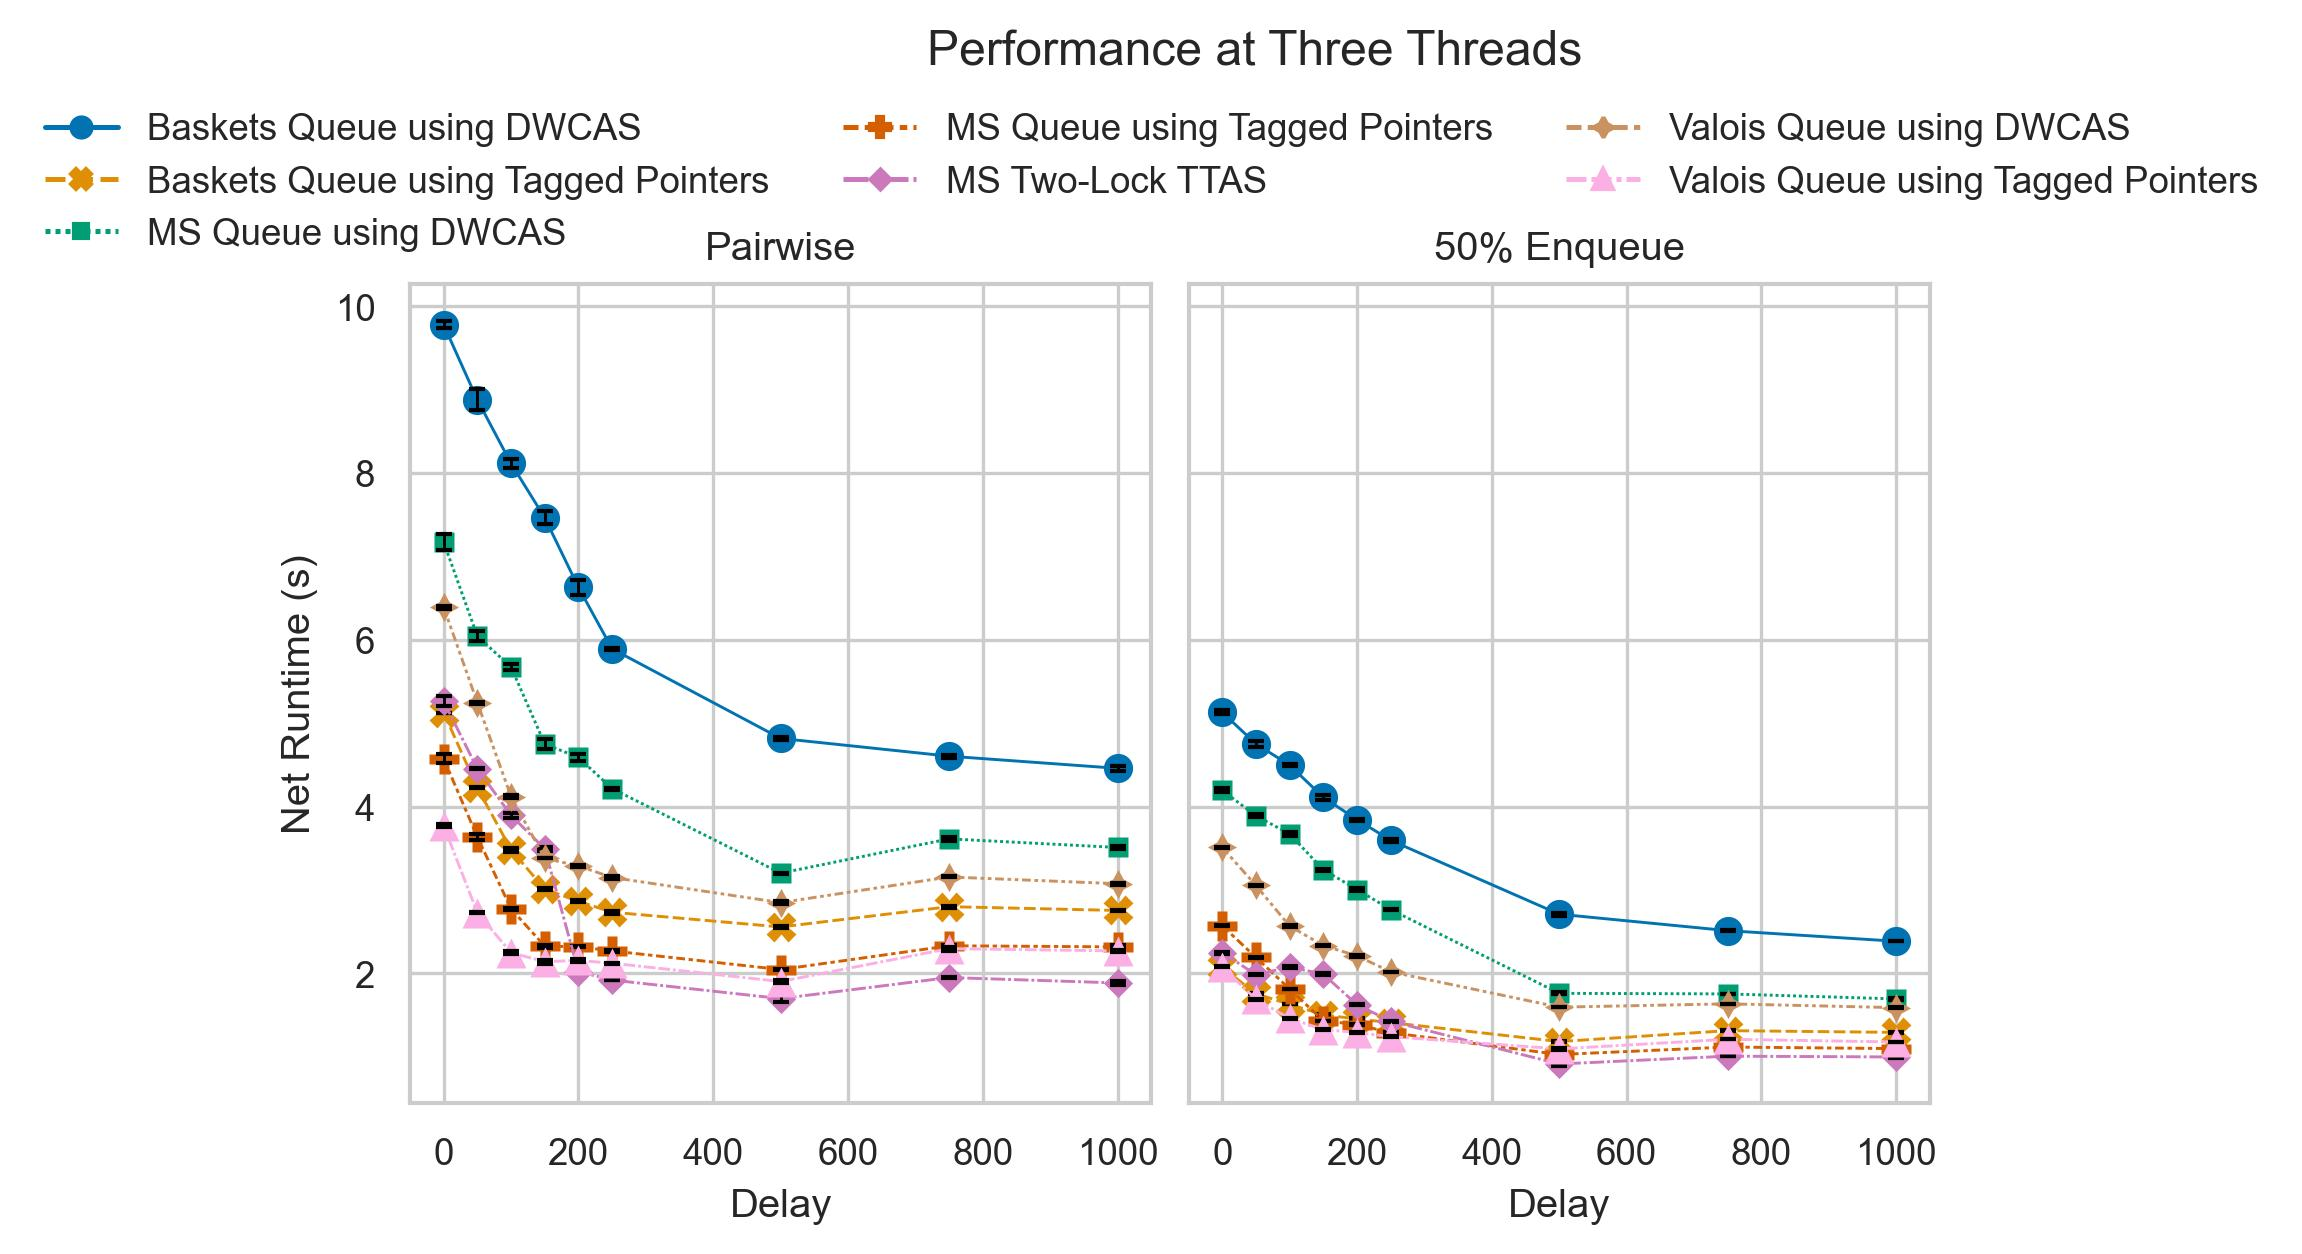
\includegraphics[width=1\textwidth]{images/plots/delay_thread_3.jpg}
    \caption{The pairwise and the 50\% benchmarks on the left and right respectively.}
    \label{fig:perf_3_thread}
\end{figure}


Up to delays of 150 nanoseconds, every non-blocking queue using tagged pointers
significantly outperforms the two-lock queue (\emph{MS-queue} is
\textbf{33.412\%} faster than the two-lock queue at 150 nanoseconds of delay),
however, as contention drops, the two-lock queue tends to become favourable. 
The \emph{MS-queue} consistently outperforms the \emph{Baskets Queue} by at least
\textbf{10.778\%}.
As the degree of contention under three threads is higher than that at two
threads, the performance penalty in using higher delays is reduced.

\begin{figure}[!ht]
    \centering
    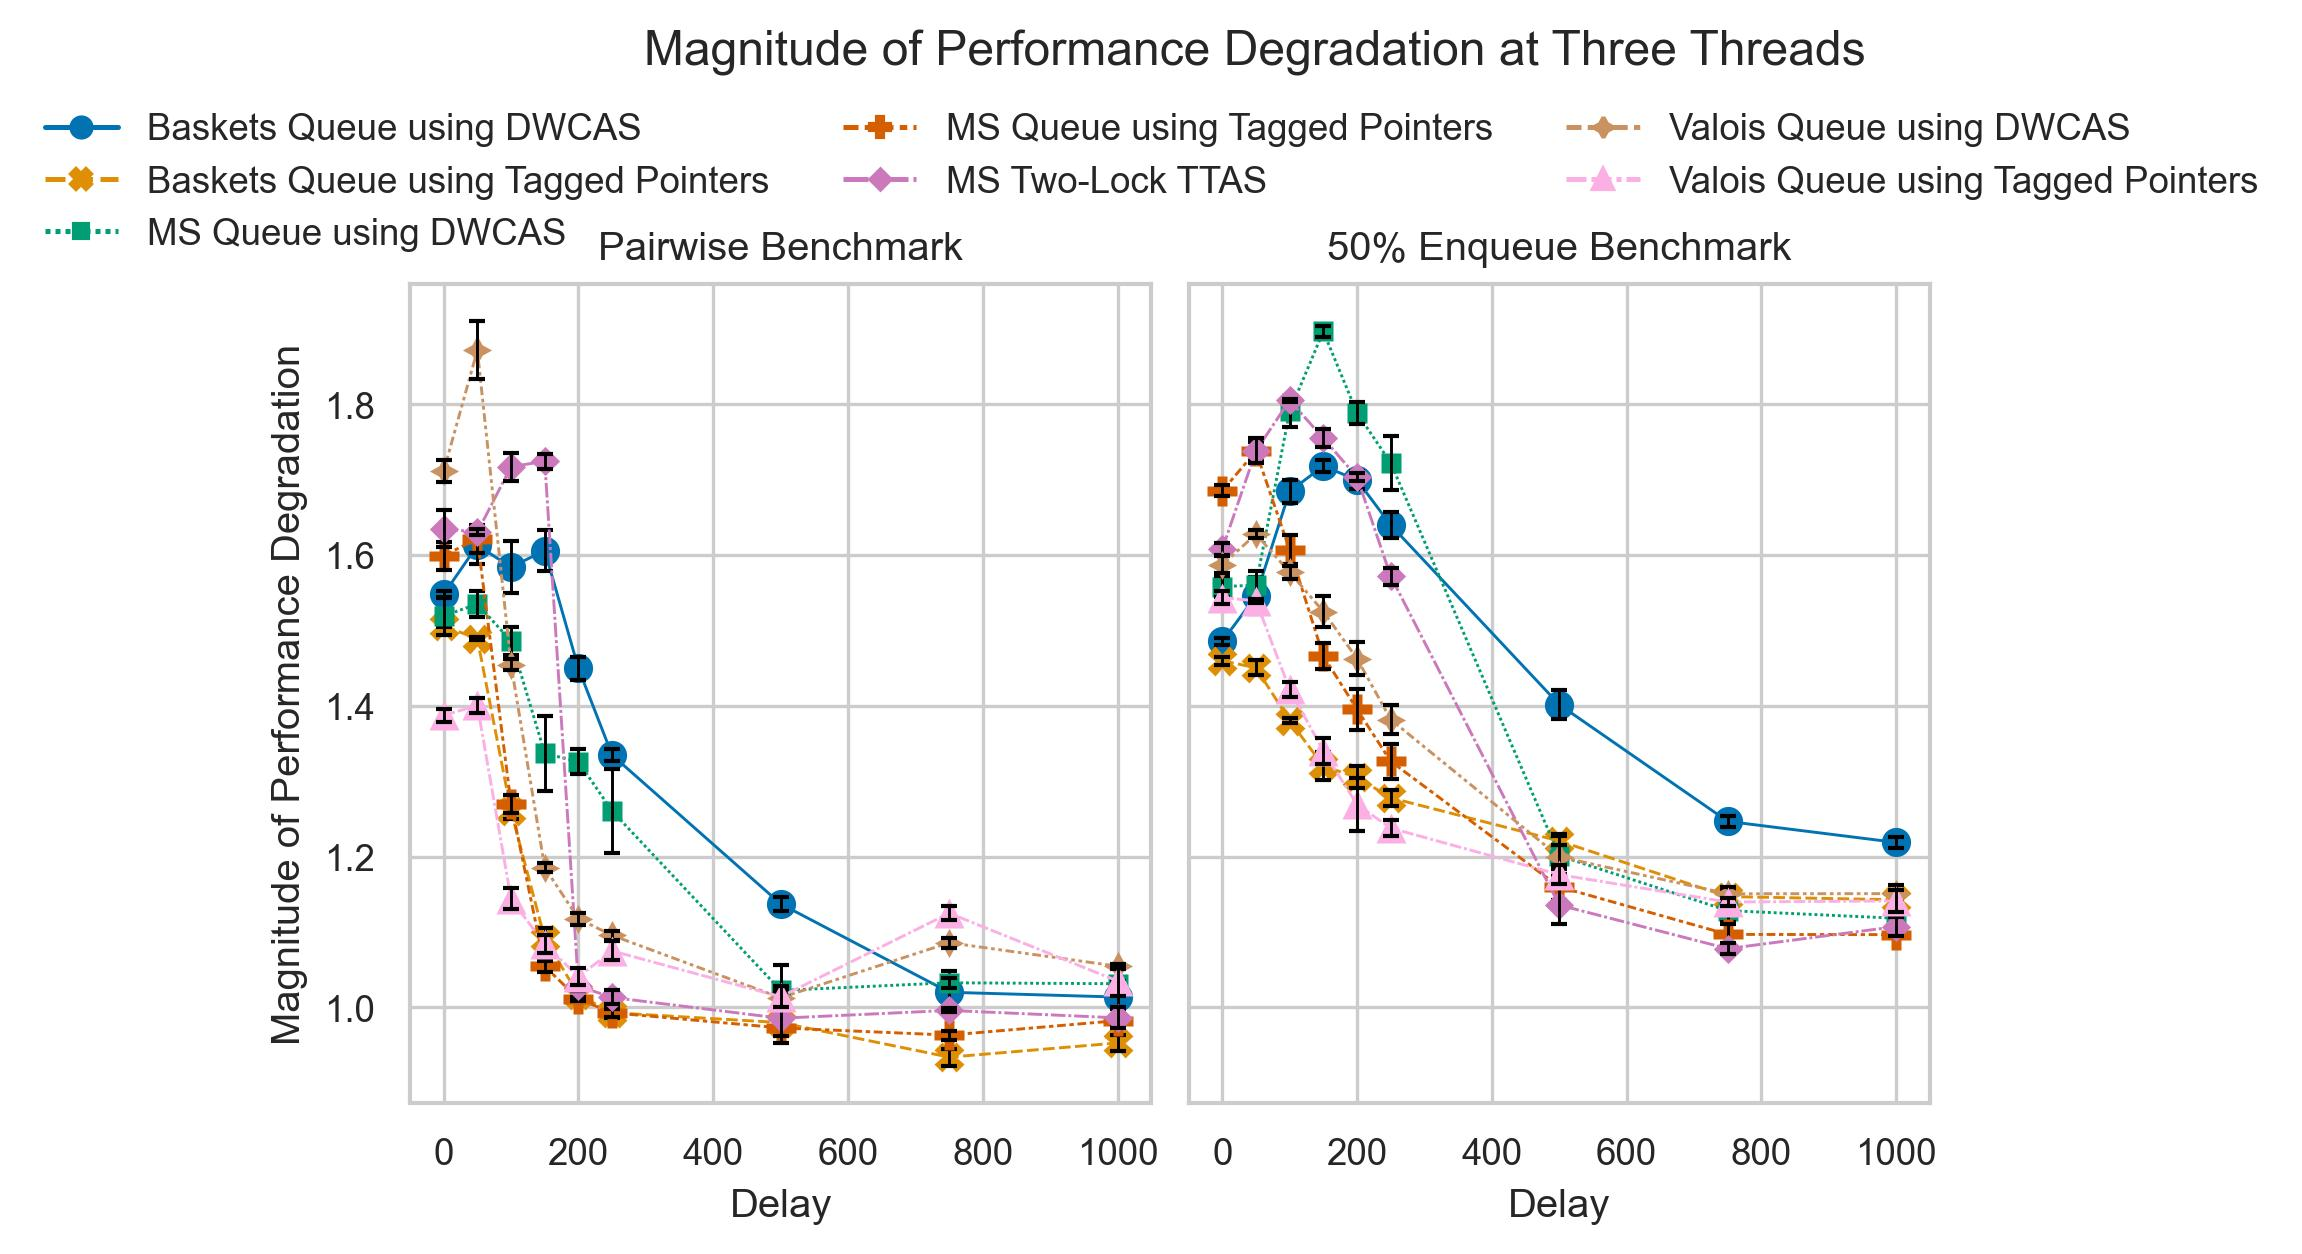
\includegraphics[width=1\textwidth]{images/plots/speedup_2.jpg}
    \caption{The pairwise and the 50\% benchmarks on the left and right respectively.}
    \label{fig:perf_deg_2_thread}
\end{figure}

\section{Workload Under Four Threads\label{sec:workload_four_threads}}

At four threads,
\citep{michael1996simple,hoffman2007baskets,ladan2008optimistic} observe a
slight dip in performance for both the \emph{MS-queue} and the \emph{Two-Lock
Queue}.
\citeauthor{hoffman2007baskets} notes an increase in performance for the
\emph{Baskets Queue}. As each queue at every delay exhibits a magnitude greater
than one, it can be concluded that performance has worsened.

Figure \ref{fig:perf_4_thread} shows that under the pairwise benchmark and no
delay, the \emph{Baskets Queue} is \textbf{0.259\%} slower than the \emph{MS-Queue};
At delays of 50 and 100 nanoseconds, the \emph{Baskets Queue} is
respectively \textbf{0.765\%} and \textbf{3.668\%} faster than the
\emph{MS-Queue}; Above delays of 100 nanoseconds, the \emph{Baskets Queue} is
up to \textbf{26.074\%} slower than the \emph{MS Queue}. 
On the other hand, the \emph{50\% Enqueue Benchmark} shows that the
\emph{Baskets Queue} is up to \textbf{42.047\%} faster than the
\emph{MS-Queue}. The distinct characteristics of the \emph{50\% Enqueue
Benchmark} allowed for the \emph{Baskets Queue} to make use of the baskets
thread-helping mechanism up to \textbf{110.964} times more than in the
\emph{Pairwise Benchmark}.
\citeauthor{hoffman2007baskets} use a variation of
\citeauthor{michael1996simple}'s \emph{pairwise benchmark}, where each thread
alternates between enqueues and dequeues. It is possible that this variation
was purposely chosen, as the alternation of operations creates an environment
where the \emph{`baskets'} mechanism is used more frequently.

% \citeauthor{hoffman2007baskets} use a variation of
% \citeauthor{michael1996simple}'s \emph{pairwise benchmark} where each thread
% alternates between executing an enqueue or a dequeue. It is possible this
% variation was purposely adopted, as the alternating execution of operations
% creates an environment where the \emph{baskets mechanism} is used more
% frequently.

\begin{figure}[!ht]
    \centering
    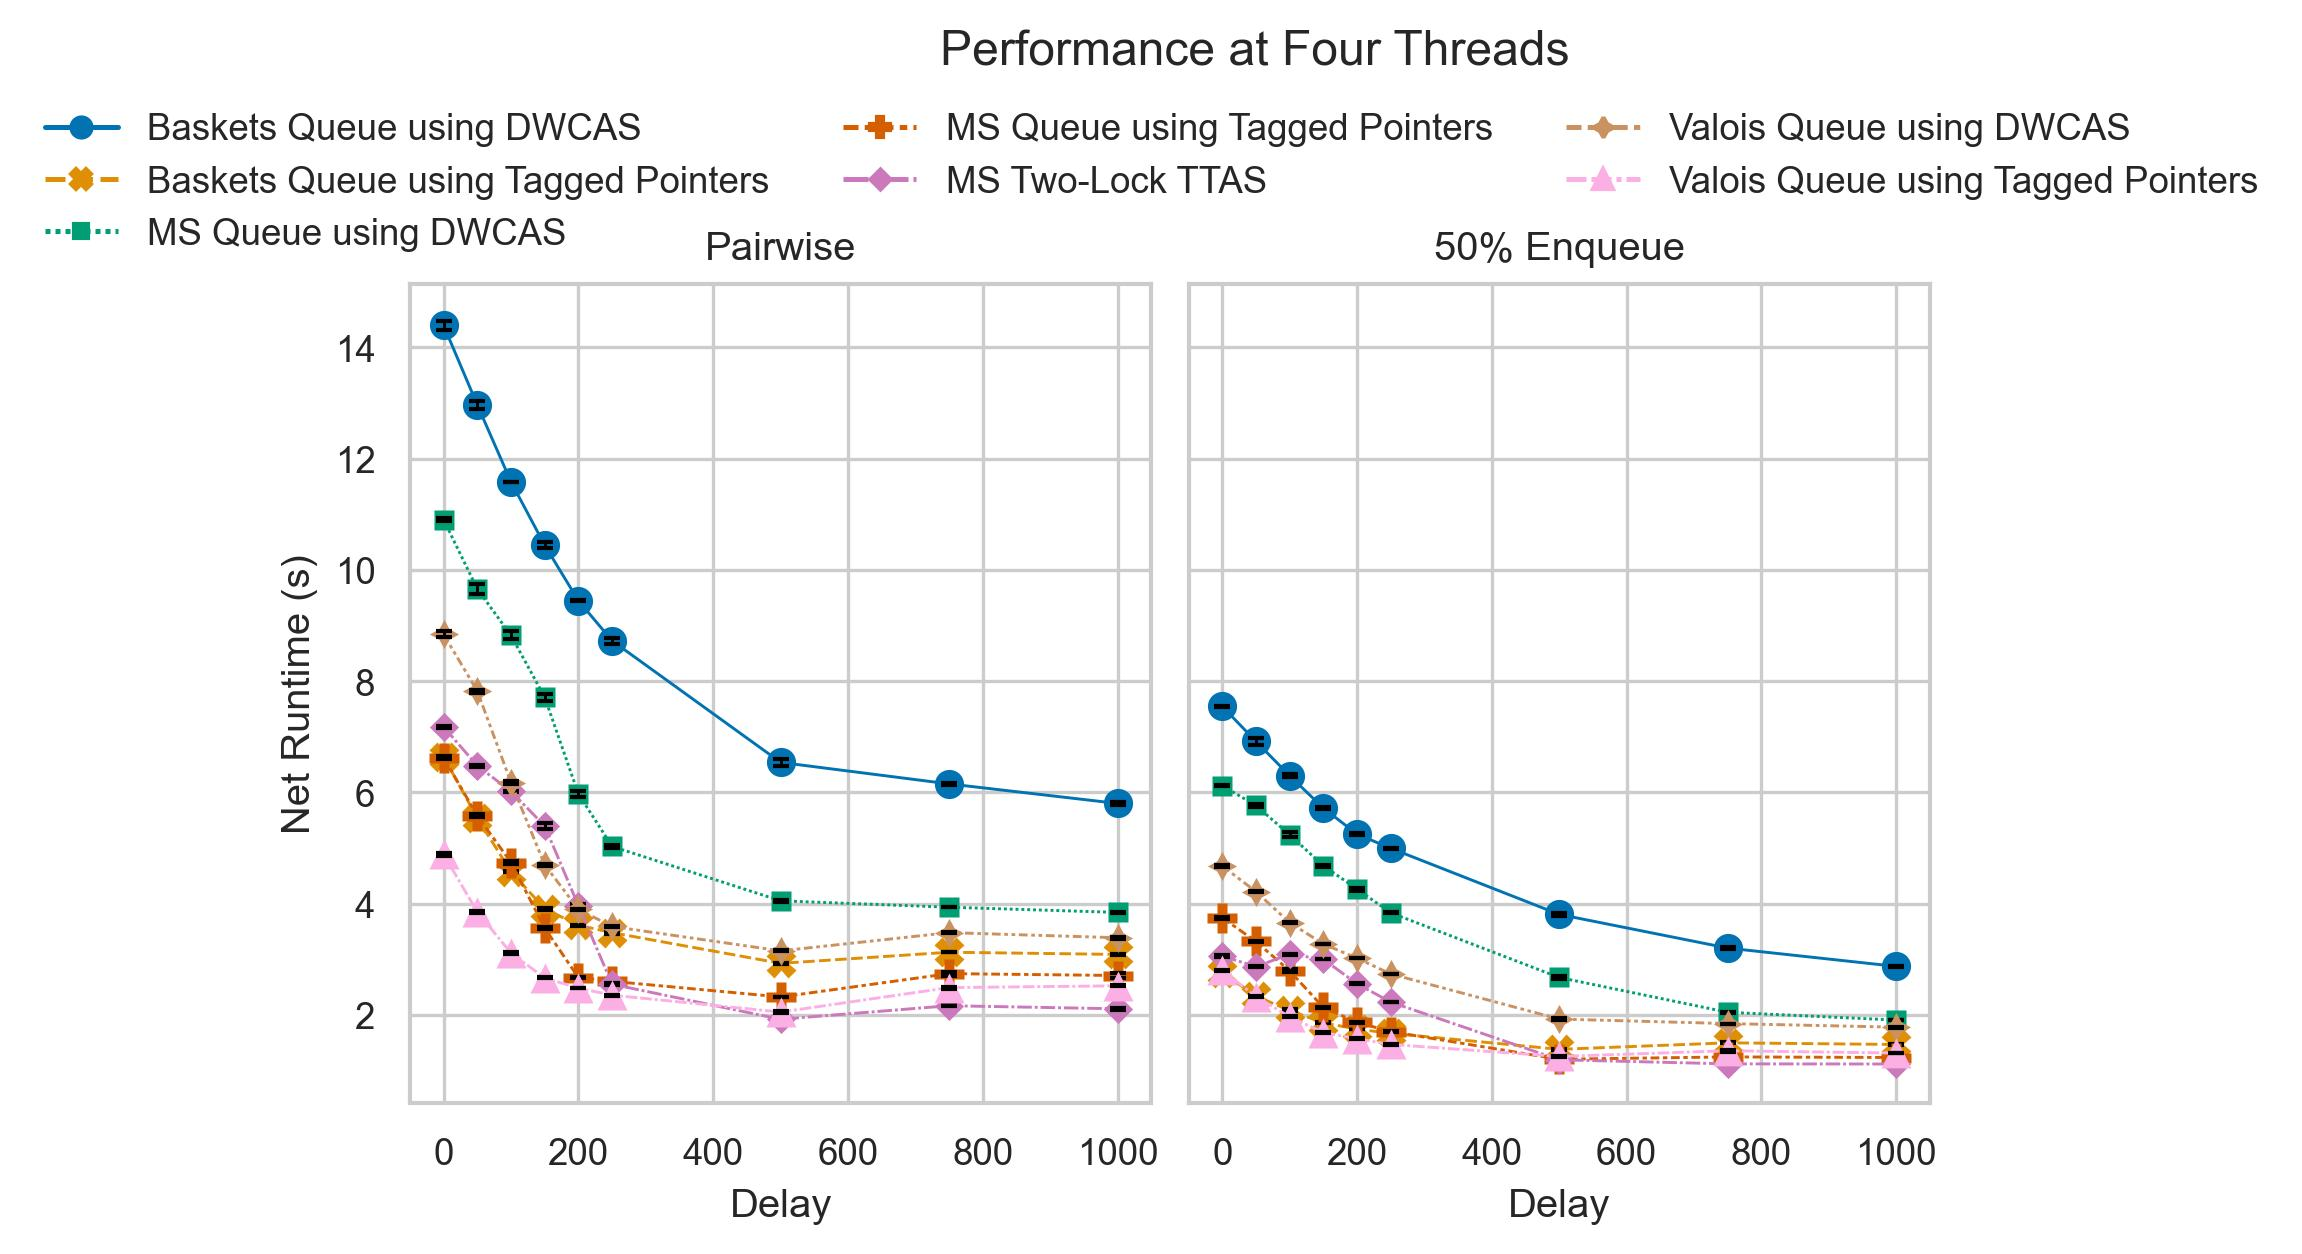
\includegraphics[width=1\textwidth]{images/plots/delay_thread_4.jpg}
    \caption{Pairwise and 50\% Enqueue Benchmarks at four threads.}
    \label{fig:perf_4_thread}
\end{figure}

\begin{figure}[!ht]
    \centering
    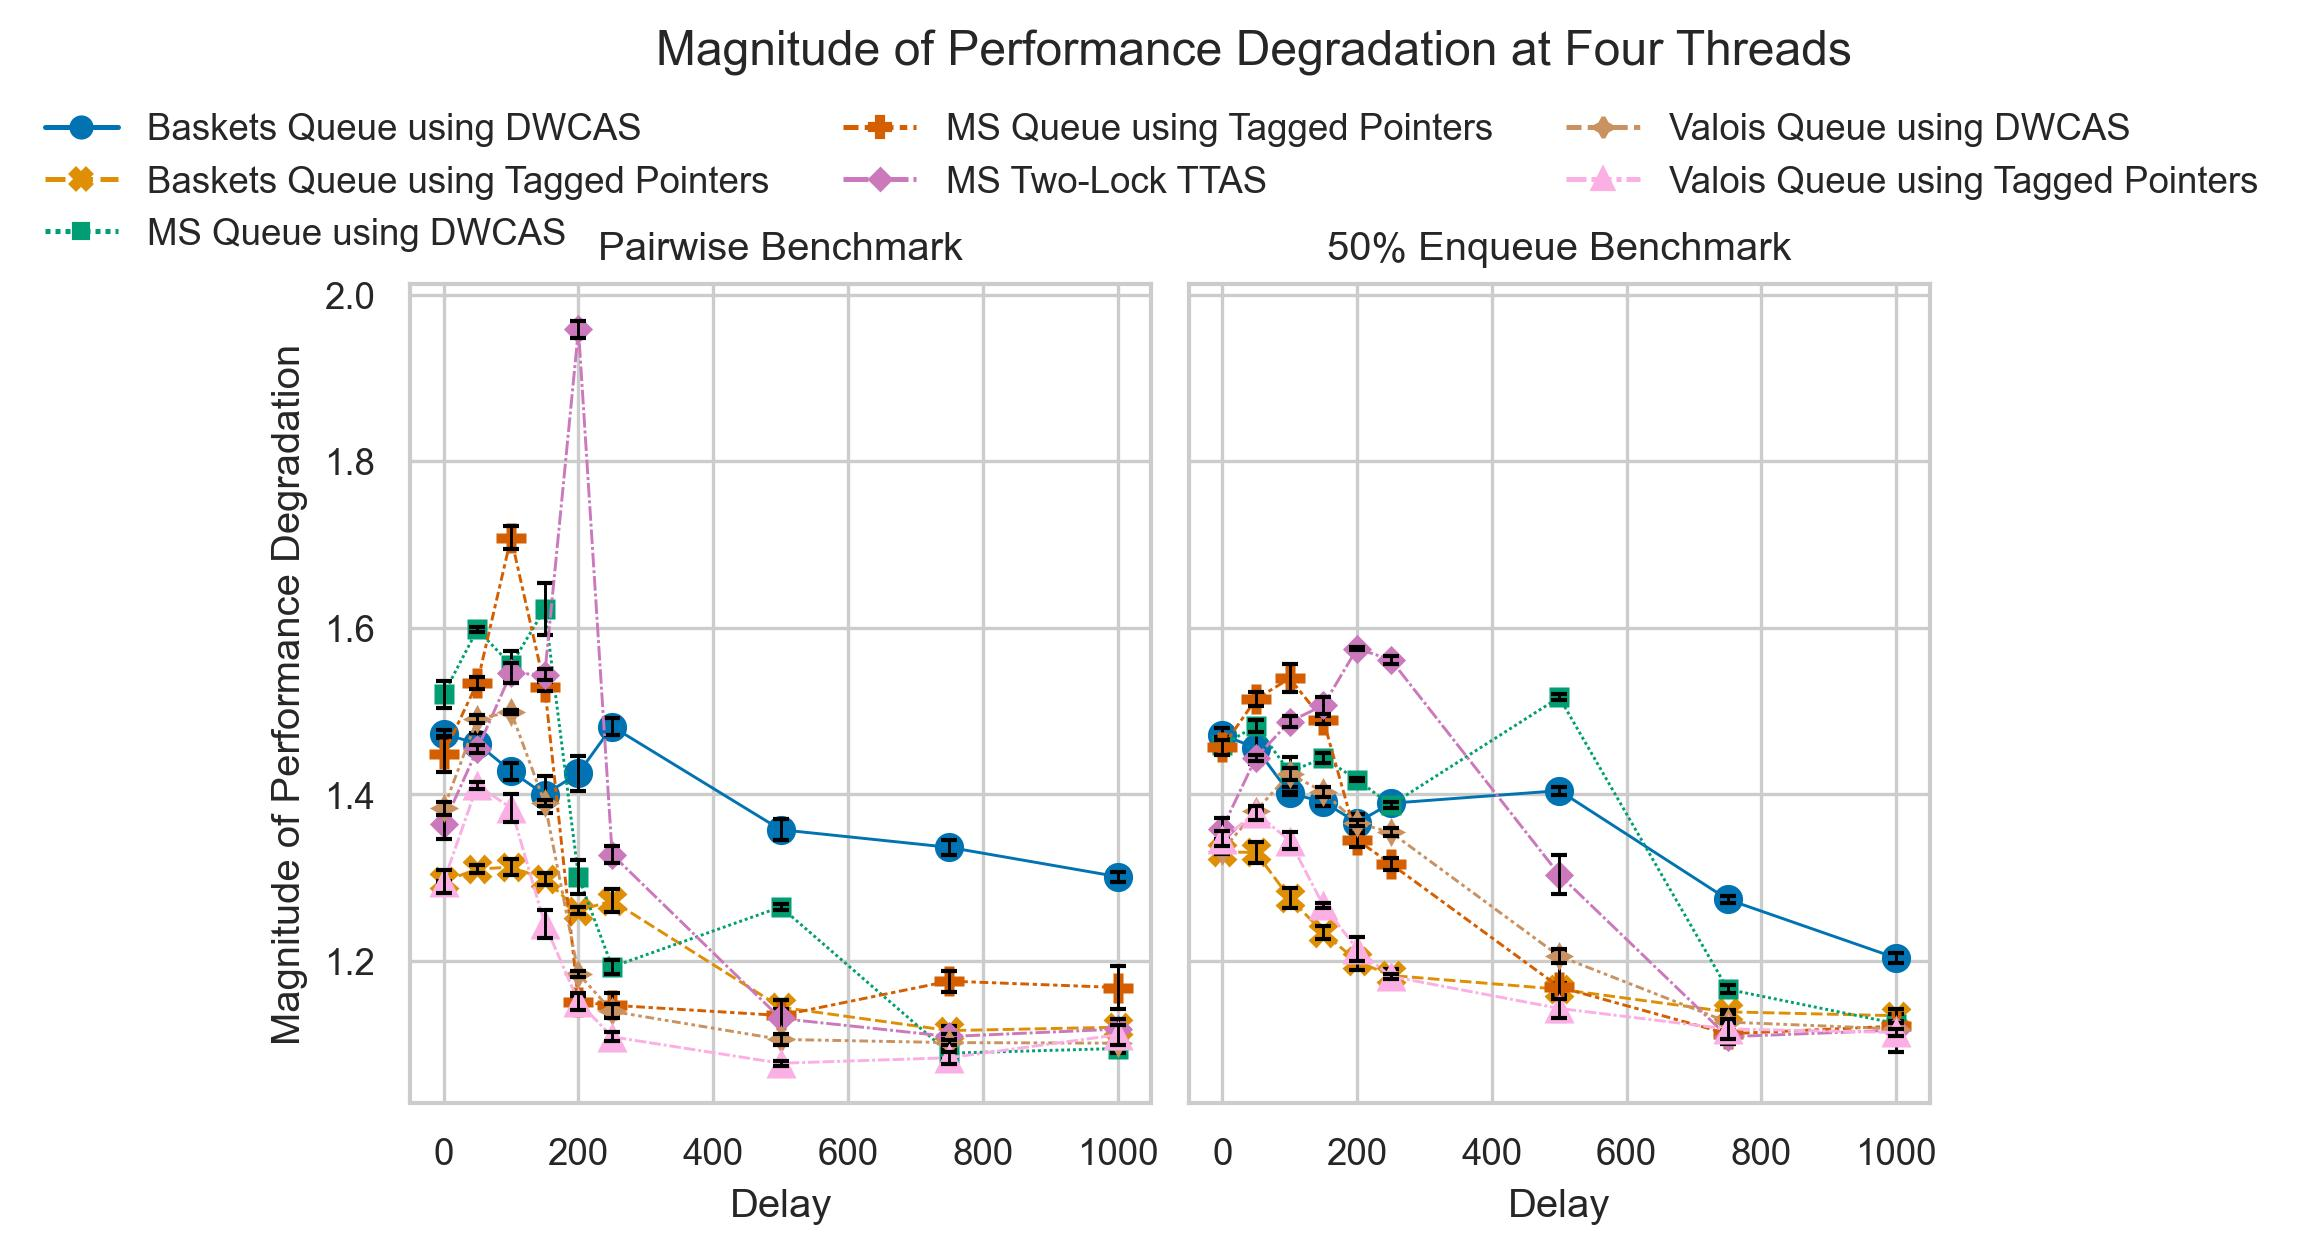
\includegraphics[width=1\textwidth]{images/plots/speedup_3.jpg}
    \caption{Degree of performance degradation at four threads.}
    \label{fig:perf_deg_4_thread}
\end{figure}

\pagebreak

\section{Performance Under Oversubscription}
\subsection{Workload Under Five Threads}
In this study, processors are oversubscribed by pinning more than one process
to each processor, forcing the thread scheduler to increase the frequency of
context-switches.

Figure \ref{fig:perf_deg_5_thread} shows that between 0 and 150 nanoseconds of delay, the
magnitude of performance degradation is a linear function of delay; As delays
greater than 150 nanoseconds are used, performance degradation explodes.
One may hypothesize that the sudden explosion in performance degradation is a result of
the significantly decreased time between context switches; as delay increases, 
the total CPU time available is further reduced.

In the pairwise benchmark, between 0 and 250 nanoseconds of delay, the \emph{Baskets
Queue} and the \emph{MS-Queue} are at most
\textbf{47.045\%} and \textbf{60.604\%} faster than the \emph{two-lock queue};
Between 500 and 1000 nanoseconds, the \emph{two-lock queue} is at most \textbf{3.351\%}
faster than the baskets queue.

Similar to the trends observed in section \ref{sec:workload_four_threads}, the \emph{Baskets
Queue} significantly outperforms the \emph{MS-Queue} (by at most \textbf{53.645\%}) only
in the \emph{50\% Enqueue Benchmark}. This repeating pattern shows that the performance of the
\emph{Baskets Queue} is heavily dependent on the utilization of the baskets mechanism.

\begin{figure}[!ht]
    \centering
    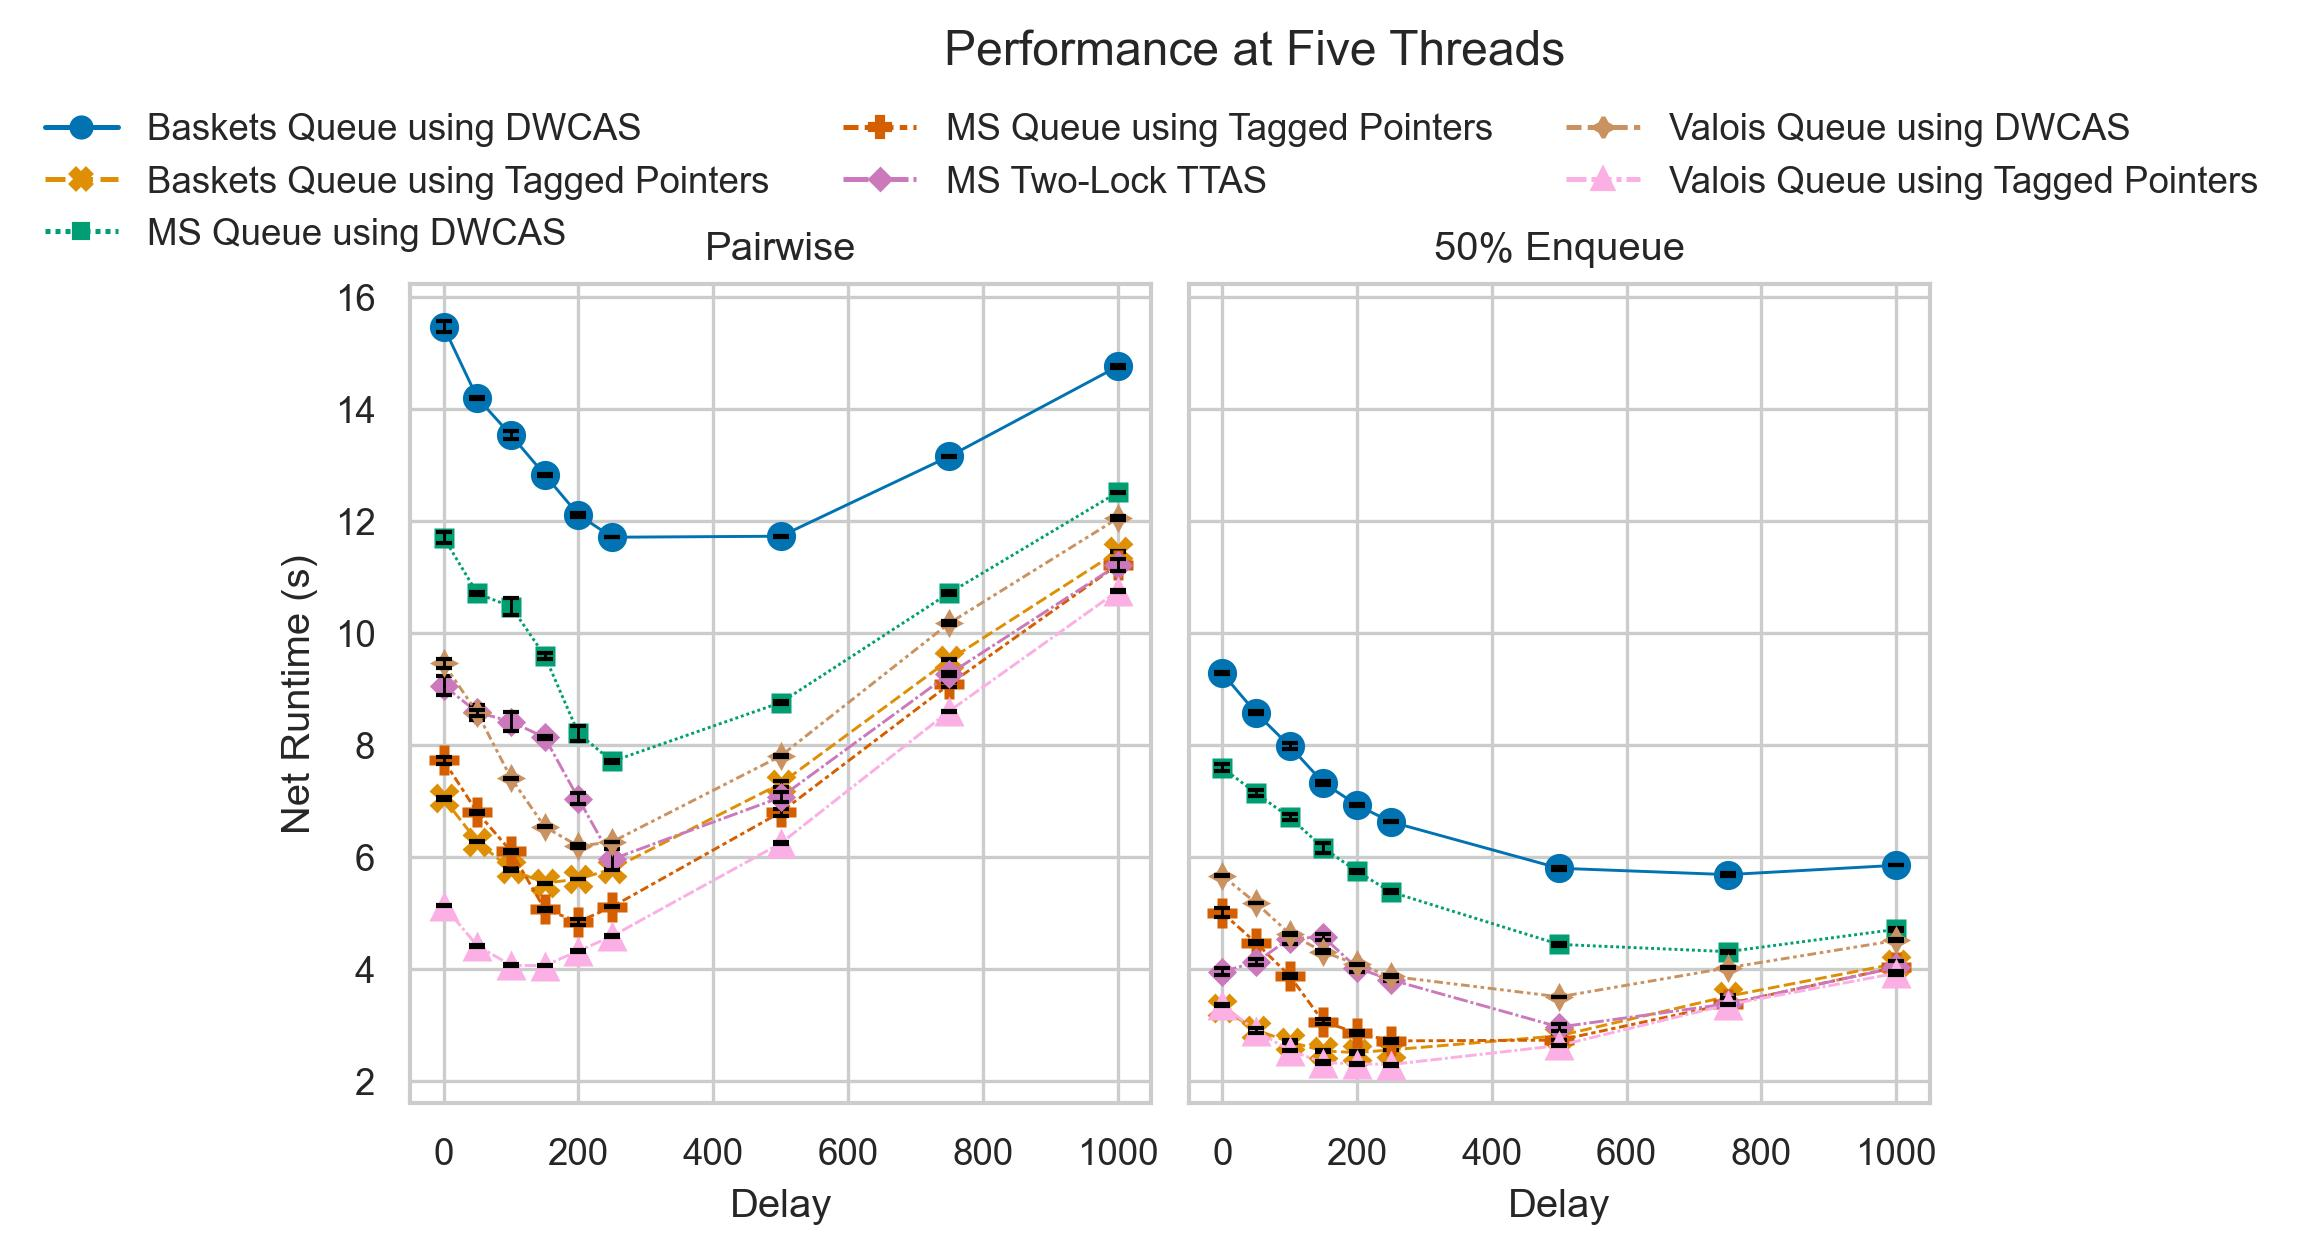
\includegraphics[width=1\textwidth]{images/plots/delay_thread_5.jpg}
    \caption{Pairwise and 50\% Enqueue Benchmarks at five threads.}
    \label{fig:perf_5_thread}
\end{figure}

\begin{figure}[!ht]
    \centering
    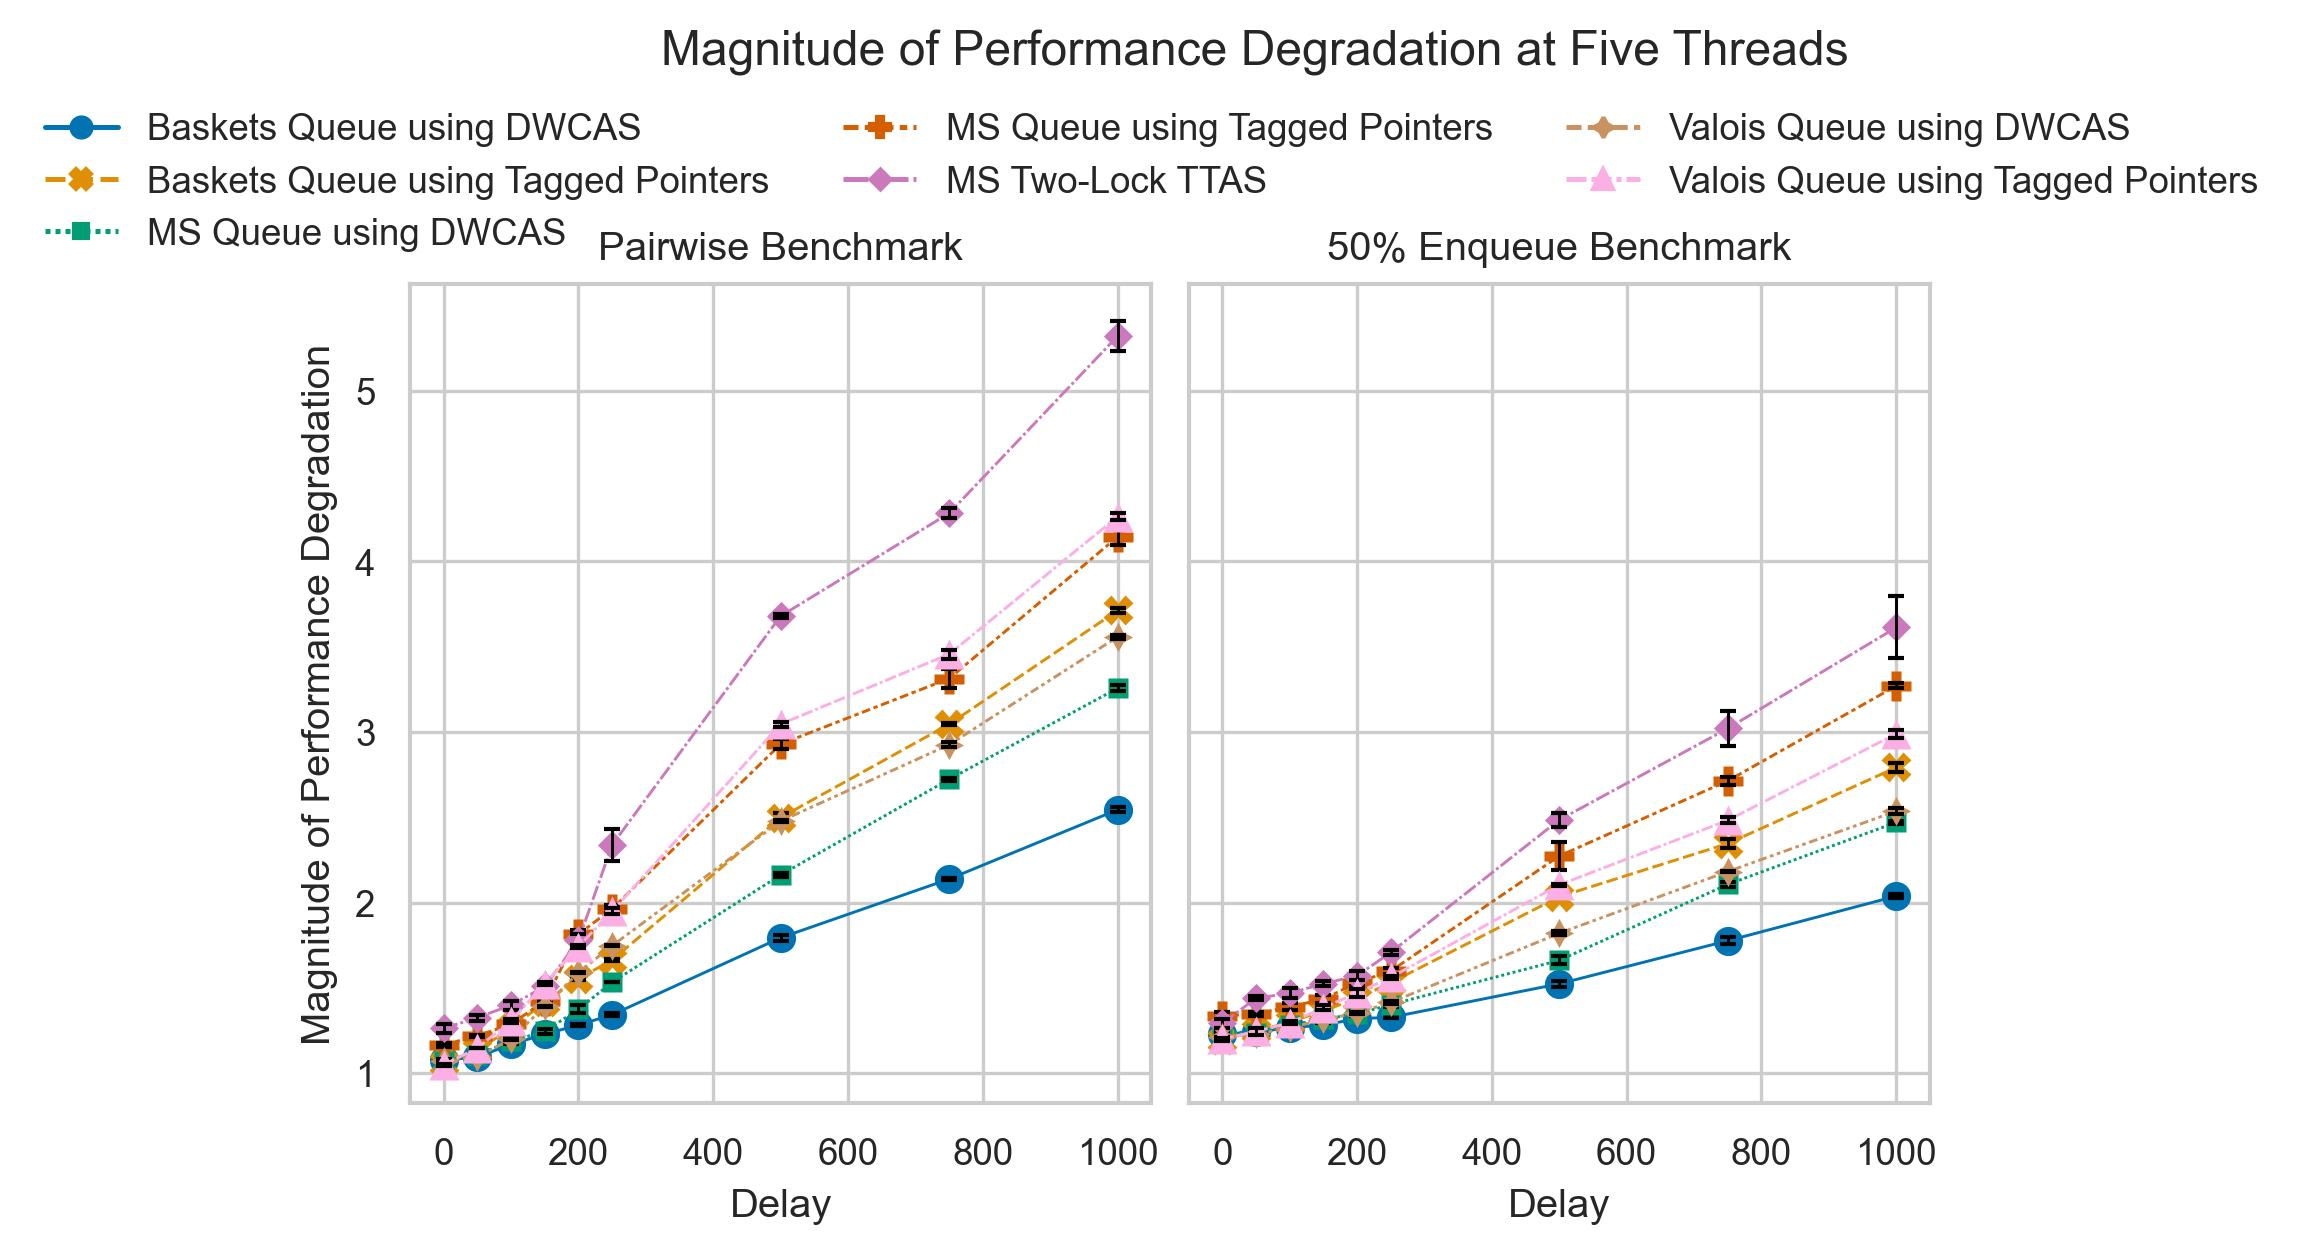
\includegraphics[width=1\textwidth]{images/plots/speedup_4.jpg}
    \caption{Degree of performance degradation at five threads.}
    \label{fig:perf_deg_5_thread}
\end{figure}

\subsection{Six Threads and Above}
At six threads, the non-blocking queues significantly outperform the \emph{two-lock}
queue at every delay. This trend repeats itself up to 12 threads, with the
degree at which the non-blocking queues outperform the \emph{two-lock queue}
increasing at every thread; the degree at which the \emph{baskets queue} outperforms
the \emph{MS-Queue} also grows with every thread.

\section{Effects of Delay on Performance}
\citeauthor{valois1995datastructures} and \citeauthor{hoffman2007baskets}
\citep{valois1995datastructures,hoffman2007baskets} note that backoff
algorithms are required to improve the efficiency of concurrent algorithms.
More often than not, a queue's optimal delay tends to be similar in consecutive
threads, with the pattern changing once over-subscription is present. Between
one and four threads, \textbf{$91.667\%$} (under the \emph{pairwise benchmark})
and \textbf{$83.333\%$} (under the \emph{50\% enqueue benchmark}) of all optimal net
runtimes have a delay of \textbf{500 nanoseconds}. Between five and twelve threads,
each queue's optimal delay slightly varies between zero and 250 nanoseconds. 

% \section{Effects of DWCAS on Concurrent Queues}
% From the data presented, one may note that employing the DWCAS instruction
% comes at a significant cost in performance. The performance penalty can be attributed to the
% latency of the DWCAS operation, leading to a lower number of operations being
% executed per second. It is possible that 

\section{Biases and Threats to Validity}
\paragraph{Artificiality of Workloads}
In \citep{gregg2014systems}, \citeauthor{gregg2014systems} claims that
\emph{micro-benchmarks} (type of benchmark adopted in this study) produces
artificial workloads, rendering results which are  solely obtained under
various assumptions. Results obtained in this study represent the concurrent
queues, whose operations are separated by fixed delays, inside a ``clean-room''
environment. Realistic workloads seldom follow such rigid patterns, making the
results' validity under real-world scenarios undetermined.

\paragraph{High Variance} Due to the quantitative nature of this study,
variance plays a major role in determining the reproducibility of the study. An
arbitrary coefficient of variance of $5\%$ was chosen as the threshold for
acceptable reproducibility. From the whole dataset, only the \emph{Baskets Queue} using Tagged Pointers at
one thread and 500 nanoseconds of delay (under the \emph{pairwise benchmark}), and
the \emph{MS Queue} using Tagged Pointers at the same number of threads and
delay (under the \emph{50\% enqueue benchmark}) had a coefficient of variance
higher than $5\%$ ($5.700\%$ and $7.424\%$ respectively). The dataset's $99\%$
quantile for coefficient of variance is \textbf{2.874\%}.

\paragraph{Lack of Benchmarking Standard} Unlike the field of
databases\textemdash concurrent queueing algorithms do not have a standardized
benchmarking methodology\textemdash allowing researchers to choose variations
of benchmarks that provide subtle biases in favour of their agenda. 

\section{Final Remarks}
This project was evaluated on a consumer-grade CPU with four cores, making
over-subscription necessary to take readings over four threads. Although this
limitation immediately affects the evaluation of this study, the benchmarking
framework aids with collecting performance data on more powerful \emph{x86\_64
Intel} CPUs.

In this study, the concurrent queueing algorithms presented in
\citep{hoffman2007baskets,valois1994datastructures,michael1996simple} were
implemented and compared with the results obtained from their seminal papers.
It was found that tagged pointers using atomic Double-Width-Compare-And-Swap (DWCAS)
instructions (for ABA prevention purposes) were several times slower than
their Single-Word-Compare-And-Swap (CAS) counterparts.

It was noted that in~\citep{michael1996simple}, \citeauthor{michael1996simple}
fail to disclose the overheads of the memory reclamation schemes used for each
queue\textemdash which if brought to light\textemdash would have shown that the
\emph{MS-Queue's} memory reclamation was simpler, and inferior to that used in
the implementation of \emph{\citeauthor{valois1994queues}' Queue} (i.e. a
reference counting system known as the \emph{safe-read} protocol).

Under single-threaded workloads, \emph{non-blocking} queues were consistently
outperformed by \citeauthor{michael1996simple}'s \emph{Two-Lock Queue}
\citep{michael1996simple}.
Workloads of two-threads present that tagged pointers using
CAS suffer from a harsher degradation in performance when compared to their
DWCAS counterpart, as they are more likely to fail a CAS, requiring one or more
retries to completely commit their changes. Yet again, the \emph{blocking
Two-Lock Queue} outperformed the \emph{non-blocking} algorithms. Similar to
prior art \citep{hoffman2007baskets,michael1996simple,ladan2008optimistic}, every
queue's net runtime increased by several times under two threads.
\citeauthor{michael1996simple} claim that speedup of less than a factor of
$\frac{1}{3}$ can be observed in the \emph{MS-Queue}, under a workload of three threads~\citep{michael1996simple},
however, similar to \citep{ladan2008optimistic,hoffman2007baskets}, the
observed speedups were more modest (up to \textbf{6.591\%}).
Under high contention at three threads, the \emph{non-blocking} queues were
superior to the \emph{blocking two-lock queue}. 
Under four threads, non-blocking queues outperform the \emph{two-lock queue} at
high contention; the \emph{Baskets Queue} only outperformed the \emph{MS-Queue}
in the \emph{50\% Enqueue Benchmark}, as it utilized the 'baskets' mechanism up
to \textbf{110.964} times more than in the \emph{Pairwise Benchmark}. Under
workloads of five threads, the CPU was oversubcribed, causing the operating
system to context-switch more frequently\textemdash reducing the CPU time slice
allocated to each thread. \emph{Non-blocking queues} remained superior at high
degrees of contention, with the \emph{blocking Two-Lock-Queue} only becoming
competitive at lower degrees of contention. Every workload with six threads or
more showed monotonically attenuating trends similar to those observed at five
threads.

A few challenges encountered in this project included minimizing interferences
created by the operating system, of a simple memory-management system which
could be used in a lock-free manner. Performance measuring tools, such as the
instrumentation of counters and the measurement of time had to be amortized
over several million iterations, as to dampen their overheads.
    \chapter{Conclusions \& Future Work}
\section{Conclusion}
Concurrent queues remain in a consistent state after being accessed
simultaneously by multiple threads. Limited work explicitly focusing on surveying concurrent
queueing algorithms exists. Consequently, we implement the algorithms
in~\citep{michael1996simple,hoffman2007baskets,valois1994queues} and compare
their performance through identical benchmarks. This study addresses the following research
objectives:

\paragraph{O1.} \emph{Implement a benchmarking framework for concurrent
queueing algorithms capable of gathering measurements similar to prior works;}

Section~\ref{sec:design_and_implementation_methodology} offers a detailed
description of the benchmarking methodologies used in this study; A high-level
overview of the benchmarking framework's design and implementation is provided in
section~\ref{sec:design_and_implementation_design_decisions}.

\paragraph{O2.} \emph{Reasonably validate the benchmarking framework through
metrics and experiments;}

Section~\ref{sec:design_and_implementation_validation} describes the efforts
taken in validating a number of the benchmarking framework's components.
The absolute error of the artificial delay (i.e.~the absolute difference
between the actual average and the expected time) and its coefficient of
variance are recorded and are kept to a minimum.
Although every queue's implementation is not thoroughly tested (due to the
complexity testing concurrent algorithms), the frequency at which specific code
paths are executed is measured; specific distributions of these counters act as
a tell-tale sign that each algorithm is either working or not working as
expected. Finally, the repeatability of the benchmarking framework is
quantified through the results' coefficient of variance, where the $99\%$
quantile of the coefficient of variance for this study is $2.874\%$

\paragraph{O3.} \emph{Implement a variety of concurrent queueing algorithms, with the aim
of replicating results from the original works;}

Four queues~\citep{valois1994queues,hoffman2007baskets,michael1996simple} (three non-blocking, and one blocking) are implemented in this
study. The non-blocking queues require tagged pointers (pointers combined with a
version counter) for ABA avoidance purposes; implementations of both 64 bit and
128 tagged pointers are presented in this study (making a total of seven
queues).

\paragraph{O4.} \emph{Critically compare each concurrent queueing algorithm's performance
under a variety of synthetic benchmarks.}

Chapter~\ref{chap:evaluation} ossifies the study by offering multi-faceted
comparisons and interpretations of each queue's performance. None of the queues
in this study were able to outperform every other queue under all
circumstances, hinting at the fact there is no such thing as a
one-size-fits-all queue. Blocking queues outperform non-blocking queues at low
levels of contention (i.e. a combination of low thread count and high delay),
however, non-blocking queues still remain competitive. At high levels of
contention, blocking queues are inferior to non-blocking ones. 

Under workloads of three threads, \citeauthor{michael1996simple} boast an
impressive speedup of a factor less than $\frac{1}{3}$~\citep{michael1996simple},
however, \citeauthor{hoffman2007baskets}'s reported speedup for the
\emph{MS-Queue}~\citep{hoffman2007baskets} and the present study's reported
speedup are more modest.

We observe trends similar
to~\citep{ladan2008optimistic,hoffman2007baskets,michael1996simple}, where
every queue experiences a significant degradation in performance under two
threads, and a small speedup at three.

\citeauthor{michael1996simple}'s evaluation~\citep{michael1996simple}
introduces significant biases in favour of their novel algorithm through the
choice of memory-reclamation schemes (effectively increasing the magnitude by
which the \emph{MS-Queue} circumstantially outperforms every other queue).

The \emph{Baskets Queue's} performance is highly dependent on the
utilization of its `baskets' mechanism, which is triggered more often under
alternating enqueues and dequeues. \citeauthor{hoffman2007baskets}~\citep{hoffman2007baskets} fail to
discover this shortcoming due to their choice of benchmarking methodologies.
Consequently, the present study is only able to replicate
\citeauthor{hoffman2007baskets}'s results under the \emph{50\% Enqueue
Benchmark}.

Between one and three threads, the \emph{MS-Queue} consistently outperforms the
\emph{Baskets Queue}, however, only under the \emph{50\% Enqueue Benchmark} does the
\emph{Baskets Queue} start to consistently outperform the \emph{MS-Queue}
at four threads or above.

Queues using 128 bit tagged pointers (through the \emph{Double-Width Compare and
Swap} instruction) are several magnitudes slower than queues adopting 64 bit
pointers.

\section{Related Work}
\citeauthor{pourmeidani2019performance}~\citep{pourmeidani2019performance} evaluates the performance of a blocking
and a non-blocking (array-based) queue on a GPU, and finds that similar to
concurrent queues on CPUs, non-blocking queues require sufficient parallelism
to outperform blocking queues.

\citeauthor{gilbert2020performance}~\citep{gilbert2020performance}
uses several open source concurrent queueing algorithms and measures
their performance with the aim of finding the queue best suited for DBMS page
evictions.

\section{Critique and Limitations}
Our evaluation is limited by the number of cores on the benchmarking
machine's CPU, although this does not affect the validity of the study, it
reduced the number of potential insights.

The queues evaluated in this study do not include memory-reclamation schemes,
potentially leading to biases.

Although several validation techniques are adopted, none of them are exhaustive
enough to ensure that from race conditions. The evaluation does not
discuss the benchmarking framework's overhead, making the degree of its effects
on the benchmarked code benchmarked unknown.

\section{Future Work}
\begin{itemize}
\item Add more algorithms with different progress conditions, such as
obstruction-free or wait-free queues.
\item Adopt \citeauthor{curtsinger2013stabilizer}'s \emph{stabilizer}~\citep{curtsinger2013stabilizer}, which allows
for statistically sound performance evaluations by forcing benchmark executions
to sample the space of memory configurations.
\item Further extend the study by running the benchmarks on machines with
better processors.
\item Add a variety of memory-reclamation schemes to the implemented queues,
discussing their effects on each queue's performance and behaviour.
\end{itemize}


%%\pagestyle{umpageback}
{%backmatter % comment this out otherwise are not numbered
    % Bibliography
    \if@openright\cleardoublepage\else\clearpage\fi
	%% For references use IEEE style [5] or Harvard style [6]
    \bibliographystyle{um-plainnat} %% specific plainnat does not show url for articles
    % Use something like https://flamingtempura.github.io/bibtex-tidy/ to clean all your bibtex entries
    {\scriptsize\bibliography{chap2/background_biblio,chap3/lit_review_related_work_biblio,chap4/design_and_implementation_biblio,chap5/evaluation_biblio,chap6/conclusions_biblio}}
	\printindex
}

\appendix
	\chapter{Source Code}
\section{Original Implementation of the MS-Queue's Memory Reclamation Scheme}

\begin{lstlisting}[language=C,caption={Memory management used in \citeauthor{michael1996simple}'s original implementation of the MS queue},label={lst:ms_queue_memory}]
void
init_memory()
{
}

unsigned
new_node()
{
  return private.node;
}

void
reclaim(unsigned node)
{
  private.node = node;
}
\end{lstlisting}

     % these are just test names as I didn't know what you'd want
	\chapter{Interfaces}
\section{Queue Interface}
\label{sec:queue_interface}
Queues are expected to implement the following seven methods found in
\emph{src/queues/queue.h}:

\begin{description}
\item bool create\_queue(void** out\_queue)
	\begin{description}
		\item[void** out\_queue] Queue to be initialized;
	\end{description}
\item bool enqueue(void* queue, void* in\_item)
	\begin{description}
		\item[void* queue] Pointer to an initialized queue;
		\item[void* in\_item] Pointer to the item that is to be enqueued;
		\item[Return] \emph{true} if enqueue is successful, else returns \emph{false}
	\end{description}
\item bool dequeue(void* queue, void** out\_item)
	\begin{description}
		\item[void* queue] Pointer to an initialized queue;
		\item[void** out\_item] - Pointer to a pointer of the variable that will be assigned the dequeued value.
		\item[Return] \emph{true} if dequeue is successful, else, if the queue is empty, or an error occurs, return \emph{false}
	\end{description}
\item void destroy\_queue(void** out\_queue)
	\begin{description}
		\item[void** out\_queue] - Pointer to a pointer of a queue that is to be de-allocated (freed).
	\end{description}
\item void register\_thread(size\_t num\_of\_iterations)
	\begin{description}
		\item This function is to be called in each thread that is used during the benchmark in order to allocate the memory necessary.
		\item[size\_t num\_of\_iterations] - The number of iterations in which the enqueue function is called, which will determine how many nodes queue elements need to be initialized for each thread.
	\end{description}
\item void cleanup\_thread()
	\begin{description}
		\item Frees the memory allocated by \emph{register\_thread}; It is the user's responsibility to call this function only after all the expected operations have been executed, as it is possible for an active thread to encounter a use-after-free error.
	\end{description}
\item char* get\_queue\_name()
	\begin{description}
		\item[Return] the name of the queue being benchmarked. The result of
    this function is appended to the results of the benchmark, in order to
    identify which results belong to a queue.
	\end{description}
\end{description}    

\section{Lock Interface}
\label{sec:lock_interface}
\begin{description}
\item[bool create\_lock(void** lock)]
\item[void destroy\_lock(void** lock)]

\item[void wait\_lock(void* lock)]
\item[void unlock(void* lock)]
\item[char* get\_lock\_name()]
\end{description}    
	% \input{appC/appendix_c_main} 
\end{document}

%%% The End %%%
